\section{Case study: Apple-Cinnamon Cheerios (Hausman 1997)}\label{sec:10-hausman}

\citet{Hausman1997} is an early study that values a single new brand with an estimated
demand system for differentiated products. It applies the virtual-price theory of \cref{sec:10-virtual} to the ready-to-eat
(RTE) cereal industry. It then adds the multiproduct pricing adjustment that \cref{sec:10-imperfect}
analyzes in general form. We take the paper in the order question, setting, data, model, identification,
results, robustness, interpretation and critique.\footnote{The NBER page of the volume is dated January
1996, so the paper is sometimes cited as Hausman (1996). Page numbers below are those of the published
volume, pp.~209--237.} \Cref{sec:10-bresnahan} then examines the comment by \citet{Bresnahan1997}, published
with the paper, which disputes both the instruments and the treatment of competition.

The paper uses several symbols that this book reserves for other objects, so we rename them. Hausman's
revenue share $s$ becomes $w$, and his margin-weighted share $w$ becomes $m$. His cost coefficient $\delta_j$
becomes $\kappa_j$, and his segment price coefficients $\delta_k$ become $b_{mg}$. His segment price indexes
$\pi_{knt}$ become $P_{gnt}$, his virtual price $p_n^*$ becomes $p_n^V$, and his elasticity $e_{kj}$ becomes
$\varepsilon_{kj}$. As in \cref{sec:10-imperfect}, elasticities in this section are signed, so own-price
elasticities are negative.

\subsection{The question}\label{sec:10-hausman-question}

Hausman asks three questions (pp.~209--210). How much consumer surplus does one incremental brand create?
By how much does the consumer price index (CPI) overstate cereal inflation because it ignores new brands?
How does multiproduct pricing by the introducing firm change the answer?

The second question motivates the first. The Bureau of Labor Statistics includes a new good in the CPI only
after it has been on sale for some time (fn.~1). The index then tracks the good's later price changes but
never records the gain from its arrival. In the terms of \cref{sec:10-virtual}, the exact index values the
new good in the base period at its virtual price, while the CPI drops the good from the base-period
comparison. Hausman quotes the agency's own warning that a systematic measurement error of this kind would
bias the measured rate of price change \citep[p.~210, quoting][]{Fixler1993}.

The question also matters for the economics of product differentiation. Hausman notes that differentiation is
one of the two basic business strategies (p.~209). He calls RTE cereal ``perhaps the foremost industry in the
introduction of new goods'' (p.~213). Some economists read cereal brand
proliferation as wasteful or as a device to deter entry \citep{Schmalensee1978}. If new brands create
little surplus, the advertising spent to launch them is mostly a private transfer. If they create large
surplus, official price indexes miss a real gain. Hausman chooses a demanding test case. Apple-Cinnamon
Cheerios (ACC), introduced by General Mills in 1989, sits next to two established brands of the same firm,
Cheerios and Honey-Nut Cheerios. Whether consumers value a product that may already be ``spanned by existing
brands'' is an empirical question (p.~216).

\subsection{The setting: brand proliferation in ready-to-eat cereal}\label{sec:10-hausman-setting}

The industry introduces many brands (pp.~213--215). From 1980 to 1992 about 190 new brands
entered a pool of about 160 existing ones. More than 95 of the new brands were discontinued. Of the 27
brands introduced in 1989, 14 had been withdrawn by 1993. Only 2 of the 190 reached a pound share above
1 percent. Even so, about 25 percent of RTE consumption came from brands introduced within the previous ten
years. Hausman notes that about 80 percent of new consumer products fail in general (fn.~9).

The industry is concentrated at the firm level and fragmented at the brand level. Six firms together
accounted for 94 percent or more of dollar sales over 1982--92 (p.~214). Kellogg's share ranged from 37.3 to
41.5 percent, General Mills' from 23.0 to 29.0 percent and General Foods' (Post) from 10.4 to 15.8 percent.
Quaker, Ralston and Nabisco each held about 3.0 to 8.9 percent, and Malt-O-Meal was the only other firm
above 1 percent. Individual brands are small. In 1993 the largest General Mills brand, Cheerios, had 5.3
percent, and the largest Kellogg brands, Frosted Flakes and Corn Flakes, had 5.0 and 4.99 percent (p.~214).

No significant manufacturer had entered successfully in fifty years. Entrants of the 1970s, such as
Pillsbury, Pet and Colgate, did not last, although real revenue grew by 6.7 percent a year over 1982--92
(p.~215). Launching a brand cost \$20--40 million in advertising and promotion in the first year, and the
spending typically continued for one or two more years. A 1 percent share counts as ``a great success''
(p.~215). The only outside competition of note came from private labels, which doubled their share from
about 4 to 8 percent over five to ten years. Ralston manufactured most of them.

Hausman rejects the view that proliferation deters entry. The Federal Trade Commission had argued this
``shared monopoly'' theory against the leading firms and lost (fn.~10). \citet{Judd1985} showed that
proliferation is a credible preemption device only if exit costs are high, and withdrawing a brand is cheap.
Hausman instead sees sunk advertising as the main barrier to entry, in the spirit of \citet{Sutton1991}. The
success of private labels, which advertise little and copy existing brands, supports this reading
(pp.~215--216). The welfare question remains open under either view. Many economists doubt the social value
of brands that mostly fail, and ACC is a natural test.

\subsection{Data}\label{sec:10-hausman-data}

The data are Nielsen Scantrak scanner data (p.~220). The time series has 137 weekly observations from
January 1990 to August 1992. The cross section has seven metropolitan areas: Boston, Chicago, Detroit,
Los Angeles, New York, Philadelphia and San Francisco. In each area Nielsen samples supermarkets by
stratified random sampling, and the sample covers most cereal sold. Sales are recorded for each stock-keeping
unit (each package size of each brand) at a weekly average price. Hausman aggregates packages to weekly
pounds of each brand and an average price per pound. The panel thus has $7 \times 137 = 959$ city-week
observations for each brand. Prices vary by about 50 percent over the sample, mostly through promotions and
coupons (pp.~216 and 228).

Brands are grouped into three segments used by industry marketing analysts (Table 5.1). The adult segment
contains Shredded Wheat Squares, Special K, Fruit Wheats, Shredded Wheat, Shredded Wheat and Bran,
Spoon-Size Shredded Wheat and Grape Nuts. The child segment contains Trix, Kix, Frosted Flakes and Froot
Loops. The family segment contains the nine brands of \cref{tab:10-hausman-desc}, ACC among them. The family
segment accounts for about 26.4 percent of RTE sales (p.~220). Hausman reports that his specification tests
do not reject the segmentation (fn.~22).

\begin{table}[htbp]
\centering
\caption{The family segment of ready-to-eat cereal, 1992}\label{tab:10-hausman-desc}
\begin{threeparttable}
\begin{tabular}{@{}llcc@{}}
\toprule
Brand & Company & \makecell{Average price\\(\$ per pound)} & \makecell{Segment share\\(percent)} \\
\midrule
Cheerios                & General Mills & 2.644 & 21.62 \\
Honey-Nut Cheerios      & General Mills & 3.605 & 15.03 \\
Apple-Cinnamon Cheerios & General Mills & 3.480 & \phantom{0}6.19 \\
Corn Flakes             & Kellogg       & 1.866 & 14.24 \\
Raisin Bran             & Kellogg       & 3.214 & 13.11 \\
Rice Krispies           & Kellogg       & 2.475 & 13.54 \\
Frosted Mini-Wheats     & Kellogg       & 3.420 & \phantom{0}9.07 \\
Frosted Wheat Squares   & Nabisco       & 3.262 & \phantom{0}1.48 \\
Raisin Bran             & Post          & 3.046 & \phantom{0}5.72 \\
\bottomrule
\end{tabular}
\begin{tablenotes}[flushleft]\footnotesize
\item Notes: Reproduced in full from \citet[Table 5.2]{Hausman1997}. Shares are shares of family-segment
sales. The three Cheerios brands together hold 42.84 percent of the segment.
\end{tablenotes}
\end{threeparttable}
\end{table}

The three Cheerios brands hold 42.84 percent of the family segment, or about 11.3 percent of all cereal
sales (p.~221). ACC holds 6.19 percent of the segment, about 1.6 percent of all cereal. By the standards of
\cref{sec:10-hausman-setting} the brand is a large success, since almost no new brand reaches 1 percent.

\subsection{A three-level demand system}\label{sec:10-hausman-model}

Hausman estimates demand with the multistage budgeting structure of \cref{sec:05-separability}, drawn in
\cref{fig:05-budget-tree}(a). The top level is total cereal demand. The middle level allocates cereal
spending across segments. The bottom level allocates segment spending across brands. Estimation proceeds
from the bottom up, and the price indexes of each level feed the level above (pp.~216--218). We index
segments by $m$ and $g$, brands by $i$ and $j$, cities by $n = 1,\dots,N$ and weeks by $t = 1,\dots,T$. In
this section $N = 7$ counts cities, not firms, and $M$ counts segments, not consumers. The subscript $n$ on
$p_n^V$ and $w_n$ still denotes the new good.

\casehead{Bottom level}
For brand $i$ in segment $m$, the share equation is an almost ideal demand system (AIDS) in segment
expenditure \citep{DeatonMuellbauer1980a},
\begin{equation}\label{eq:10-h-bottom}
  w_{int} = \alpha_{in} + \beta_i\ln\frac{Y_{mnt}}{P_{mnt}} + \sum_{j\in m}\gamma_{ij}\ln p_{jnt} + \xi_{int}
\end{equation}
(Hausman's eq.~5). Here $w_{int}$ is the revenue share of brand $i$ in segment spending $Y_{mnt}$, and
$P_{mnt}$ is the segment price index. The price per pound of brand $j$ is $p_{jnt}$, and $\xi_{int}$ is the
demand error. The intercept $\alpha_{in}$ is a brand-city effect. Table 5.3 shows that the equations also
include a quadratic time trend and a display variable $\ln(DISP + 1)$. Adding up across the brands of the
segment requires $\sum_i\alpha_{in} = 1$, $\sum_i\beta_i = 0$ and $\sum_i\gamma_{ij} = 0$. Homogeneity requires
$\sum_j\gamma_{ij} = 0$, and Slutsky symmetry requires $\gamma_{ij} = \gamma_{ji}$.

Three features of \eqref{eq:10-h-bottom} carry the analysis. First, the $\gamma_{ij}$ are unrestricted apart
from symmetry and homogeneity. With nine brands that leaves $\frac{9\times 8}{2} = 36$ free price coefficients,
and no equal-cross-elasticity assumption constrains substitution within the segment. Second, a test of
$\beta_i = 0$ for all $i$ is a test of \emph{segment homotheticity}, the hypothesis that brand shares do not
depend on segment spending. Third, the expenditure variable is segment spending. Using total spending ``is
inconsistent with the economic theory of multistage budgeting'' and gives worse results (p.~217).

The \emph{conditional elasticities} hold segment spending fixed. With the translog index of the AIDS,
Shephard's lemma gives $\frac{\partial\ln P_{m}}{\partial\ln p_j} = w_{j|m} - \beta_j\ln\frac{Y_m}{P_m}$, where
$w_{j|m}$ is brand $j$'s share of the segment. Since $q_i = \frac{w_{i|m}Y_m}{p_i}$, we have
$\ln q_i = \ln w_{i|m} + \ln Y_m - \ln p_i$. Differentiating with respect to $\ln p_j$ at fixed $Y_m$,
\begin{align}
  \varepsilon^c_{ij} &= -\indic\{i = j\} + \frac{1}{w_{i|m}}\frac{\partial w_{i|m}}{\partial\ln p_j}\notag\\
  &= -\indic\{i = j\} + \frac{\gamma_{ij} - \beta_i\bigl(w_{j|m} - \beta_j\ln\frac{Y_m}{P_m}\bigr)}{w_{i|m}}.
  \label{eq:10-h-cond-elast}
\end{align}
Differentiating instead with respect to $\ln Y_m$ gives the conditional expenditure elasticity
$\phi_{i|m} = 1 + \frac{\beta_i}{w_{i|m}}$. These are the AIDS formulas of \cref{sec:05-aids-elasticities},
written with within-segment shares.

\casehead{Middle level}
Segment quantities follow a log-log system,
\begin{equation}\label{eq:10-h-middle}
  \ln q_{mnt} = \alpha_{mn} + \phi_m\ln Y_{nt} + \sum_{g=1}^{M}b_{mg}\ln P_{gnt} + \xi_{mnt}, \qquad m = 1,\dots,M
\end{equation}
(Hausman's eq.~6). Here $q_{mnt}$ is the pound volume of segment $m$, $Y_{nt}$ is total cereal spending in
the city-week, and $P_{gnt}$ is the price index of segment $g$. Because cereal spending is held fixed,
$\phi_m$ is the segment's expenditure elasticity and $b_{mg}$ are price elasticities conditional on cereal
spending. Hausman uses Stone indexes at this level (p.~221) and states that the choice between exact and
Stone indexes typically matters little (p.~218). Exact two-stage budgeting requires additive separability at the level above, and the
AIDS is a generalized Gorman polar form, so Gorman's theorem applies \citep[fn.~17]{Hausman1997}. A less
restrictive middle level, not consistent with exact two-stage budgeting, gives similar results (fn.~17).
The log-log system is second-order flexible, and Slutsky restrictions are not imposed on it (fn.~18).

\casehead{Top level}
Total cereal consumption $Q_t$ satisfies
\begin{equation}\label{eq:10-h-top}
  \ln Q_t = a_0 + a_1\ln y_t + \varepsilon_U\ln\Pi_t + Z_t\psi + \xi_t
\end{equation}
(Hausman's eq.~7), where $y_t$ is real disposable income, $\Pi_t$ is the real cereal price index and $Z_t$
holds demographic and monthly seasonal variables. A longer period than store data provide helps to estimate
this elasticity, so Hausman fits \eqref{eq:10-h-top} to sixteen years of national monthly data from the Bureau
of Labor Statistics. He uses
instrumental variables, with cost shifters for ingredients, packaging and labor as instruments (p.~218). The
coefficient $\varepsilon_U$ is the price elasticity of total cereal demand.

\casehead{Combining the levels}
Pricing and welfare calculations need \emph{unconditional} elasticities, which let segment and cereal
spending respond to prices. The next result writes them in terms of the three levels. It is the formula of
\eqref{eq:05-hlz-uncond} for beer, restated in this section's notation with Stone indexes. We restate it
because its rank-one structure matters for reading Hausman's tables.

\begin{proposition}[Unconditional elasticities in a three-level system]\label{prop:10-elasticity-aggregation}
Let brand $i$ belong to segment $m$ and brand $j$ to segment $g$. Assume the following.
\begin{enumerate}[label=(\roman*)]
\item The demand $q_i$ depends on prices only through the prices of segment $m$ and on spending only through
$Y_m$, with elasticities $\varepsilon^c_{ij}$ and $\phi_{i|m}$.
\item Segment spending is $Y_m = P_mq_m$, with a Stone index satisfying
$\frac{\partial\ln P_g}{\partial\ln p_j} = w_{j|g}$.
\item Segment quantities follow \eqref{eq:10-h-middle}.
\item Cereal spending is $Y = \Pi Q$, with $\ln\Pi = \sum_g w_g\ln P_g$ and $w_g$ segment $g$'s share of cereal
spending. Cereal volume $Q$ follows \eqref{eq:10-h-top} at fixed income.
\end{enumerate}
Then
\begin{equation}\label{eq:10-elasticity-aggregation}
  \varepsilon_{ij} = \indic\{m = g\}\,\varepsilon^c_{ij}
  + \phi_{i|m}\,w_{j|g}\bigl[\indic\{m = g\} + b_{mg} + \phi_m(1 + \varepsilon_U)w_g\bigr].
\end{equation}
\end{proposition}

\begin{proof}
Write $q_i = q_i^c(p_m, Y_m)$. The price $p_j$ moves $q_i$ directly if $j$ is in segment $m$, and indirectly
through $Y_m$. By the chain rule,
\begin{equation*}
  \varepsilon_{ij} = \indic\{m = g\}\,\varepsilon^c_{ij} + \phi_{i|m}\frac{\dd\ln Y_m}{\dd\ln p_j}.
\end{equation*}
By (ii), $\ln Y_m = \ln P_m + \ln q_m$. The index $P_m$ responds to $p_j$ only if $m = g$, so
\begin{equation*}
  \frac{\dd\ln Y_m}{\dd\ln p_j} = \indic\{m = g\}\,w_{j|g} + \frac{\dd\ln q_m}{\dd\ln p_j}.
\end{equation*}
By (iii), $q_m$ responds to $p_j$ through the index $P_g$ and through cereal spending $Y$:
\begin{equation*}
  \frac{\dd\ln q_m}{\dd\ln p_j} = b_{mg}\,w_{j|g} + \phi_m\frac{\dd\ln Y}{\dd\ln p_j}.
\end{equation*}
By (iv), $\ln Y = \ln\Pi + \ln Q$ and $\frac{\partial\ln\Pi}{\partial\ln p_j} = w_g\,w_{j|g}$. With income fixed,
$\frac{\dd\ln Q}{\dd\ln p_j} = \varepsilon_U\,w_g\,w_{j|g}$, so
\begin{equation*}
  \frac{\dd\ln Y}{\dd\ln p_j} = (1 + \varepsilon_U)\,w_g\,w_{j|g}.
\end{equation*}
Substituting the last display into the one before it, and that into the second display,
\begin{equation*}
  \frac{\dd\ln Y_m}{\dd\ln p_j} = w_{j|g}\bigl[\indic\{m = g\} + b_{mg} + \phi_m(1 + \varepsilon_U)w_g\bigr].
\end{equation*}
Inserting this into the first display gives \eqref{eq:10-elasticity-aggregation}.
\end{proof}

Two implications follow. Within a segment ($m = g$), the gap between unconditional and conditional
elasticities is $\phi_{i|m}\,w_{j|m}\,B_m$, with a common factor
$B_m = 1 + b_{mm} + \phi_m(1 + \varepsilon_U)w_m$. The matrix of gaps is therefore the outer product of the
vector of expenditure elasticities and the vector of shares, a matrix of rank one. Across segments only the
expenditure channel remains, so all brand-specific substitution between segments is ruled out. For the
family segment, Table 5.4 gives $b_{FF} = -1.829$ and $\phi_F = 0.999$. With $\varepsilon_U = -0.90$ and
$w_F = 0.264$ the factor is $B_F = 1 - 1.829 + 0.999 \times 0.10 \times 0.264 = -0.80$. A higher price of any
family brand raises the segment index, and because segment demand is elastic, family spending falls.

\subsection{Identification and estimation}\label{sec:10-hausman-identification}

Prices in \eqref{eq:10-h-bottom} are endogenous if retailers or manufacturers set them knowing local demand.
The usual remedy, input prices excluded from demand, fails here. There may be too few input prices, and they
are rarely observed weekly (p.~219). Hausman exploits the panel structure instead. He models the price of
brand $j$ in city $n$ and week $t$ as
\begin{equation}\label{eq:10-h-price}
  \ln p_{jnt} = \kappa_j\ln c_{jt} + \mu_{jn} + \omega_{jnt}
\end{equation}
(Hausman's eq.~8). The cost $c_{jt}$ has no city-specific time variation, consistent with national shipping
and national advertising. The effect $\mu_{jn}$ captures city-specific transport costs and wages. The shock
$\omega_{jnt}$ has mean zero and captures local promotions. \Cref{sec:05-hlz-identification} writes the same
model as \eqref{eq:05-hlz-price} for the beer study of \citet{HausmanLeonardZona1994}.

\begin{assumption}[Independence across cities]\label{ass:10-hausman-iv}
After brand-city effects are removed, the following hold.
\begin{enumerate}[label=(\roman*)]
\item The shocks $\omega_{jnt}$ are independent across cities. They may be correlated across brands within a
city \citep[fn.~19]{Hausman1997}.
\item The demand errors $\xi_{int}$ are uncorrelated with the cost component $c_{jt}$ and with the price
shocks $\omega_{j\ell t}$ of every other city $\ell\neq n$.
\end{enumerate}
\end{assumption}

Let a tilde denote the deviation from the brand-city mean. Under \cref{ass:10-hausman-iv} the prices of every
segment brand in other cities are valid instruments,
\begin{equation}\label{eq:10-h-moment}
  \E\bigl[\widetilde{\ln p}_{j\ell t}\,\tilde\xi_{int}\bigr] = 0, \qquad i, j\in m,\ \ell\neq n.
\end{equation}
Relevance comes from the common cost. By \eqref{eq:10-h-price},
$\Cov(\widetilde{\ln p}_{j\ell t},\widetilde{\ln p}_{jnt}) = \kappa_j^2\Var(\widetilde{\ln c}_{jt})$, which is
positive whenever national costs vary over time. In Hausman's words, prices in one city, ``after elimination
of city- and brand-specific effects'', are driven by underlying costs (p.~219). This is the logic of
\citet{HausmanTaylor1981} and \citet{BreuschMizonSchmidt1989}: after unit effects are removed, variation
shared with other units serves as an instrument. With more than two cities the model is overidentified, and
the restrictions can be tested (fn.~20). Instruments of this kind are now called \emph{Hausman instruments}.
\Cref{sec:05-hlz-identification} discusses them in general, and \cref{ch:blp} uses them in random-coefficient
models.

Hausman offers a second interpretation (p.~219). Suppose supermarkets set weekly prices under constant
short-run marginal cost and do not adjust them to clear the market. Then prices are predetermined with
respect to the demand errors, and instruments are unnecessary for prices. Segment spending $Y_{mnt}$ may still
need instruments, because it responds to the same demand shocks. The choice between the two views can be
tested with the specification test of \citet{Hausman1978}.

\casehead{Estimator}
Stack the share equations of the segment, dropping one by adding up (Post Raisin Bran in Table 5.3). For
city $n$ and week $t$ let $\xi_{nt}(\theta)$ be the vector of residuals of the remaining eight equations and
$Z_{nt}$ the vector of instruments: the exogenous regressors and the other-city prices. The estimator
combines seemingly unrelated regression with instruments (p.~221). In generalized method of moments form it
solves
\begin{equation}\label{eq:10-h-gmm}
  \hat\theta = \argmin_{\theta}\;
  \Bigl[\sum_{n,t}\xi_{nt}(\theta)\otimes Z_{nt}\Bigr]^\top
  \Bigl[\hat\Sigma\otimes\sum_{n,t}Z_{nt}Z_{nt}^\top\Bigr]^{-1}
  \Bigl[\sum_{n,t}\xi_{nt}(\theta)\otimes Z_{nt}\Bigr]
\end{equation}
subject to symmetry, with $\hat\Sigma$ a first-step estimate of the covariance matrix of the eight errors.
This is a form of three-stage least squares, and \cref{app:econometrics} develops the general theory. Hausman tests
and imposes symmetry, which is not rejected, and tests homotheticity, which is rejected (p.~221). The
paper does not report the instrument list in full, the first-stage fit, or the outcome of the
overidentification and Hausman tests.

The source of identifying variation deserves emphasis. After brand-city effects are removed, the slope of
each brand's demand curve is identified by the weekly co-movement of that brand's price across the seven
cities. Hausman attributes this co-movement to national costs. Any national demand shock that also moves
prices in all cities in the same week contaminates it. \Cref{sec:10-bresnahan} works out the consequences.

\subsection{Estimates}\label{sec:10-hausman-estimates}

\Cref{tab:10-hausman-aids} reproduces the price, expenditure and display coefficients of the bottom level.
Own-price coefficients are large and precise. Most cross-price coefficients are positive, as substitution
suggests. The three Cheerios brands are substitutes for each other: $\gamma_{12} = 0.02087$,
$\gamma_{13} = 0.00842$ and $\gamma_{23} = 0.01849$, each more than two standard errors from zero. A few cross
coefficients are negative, such as $\gamma_{56} = -0.00791$ between Kellogg's Raisin Bran and Rice Krispies.
The expenditure coefficients show that homotheticity fails. ACC's $\beta_3 = -0.00854$ implies an
expenditure elasticity within the segment of $1 + \frac{-0.00854}{0.06193} = 0.86$. Corn Flakes and Rice
Krispies, with positive $\beta_i$, have elasticities above one. Display coefficients are positive for all brands
and significant for all but Rice Krispies.

\begin{table}[htbp]
\centering
\caption{Bottom-level AIDS estimates for the family segment (selected coefficients)}\label{tab:10-hausman-aids}
\begin{threeparttable}
\footnotesize
\setlength{\tabcolsep}{3.2pt}
\begin{tabular}{@{}lcccccccc@{}}
\toprule
 & (1) & (2) & (3) & (4) & (5) & (6) & (7) & (8) \\
 & Cheerios & HN Ch. & AC Ch. & Corn Fl. & K Rais. B. & Rice Kr. & Fr. Mini-W. & Fr. Wh. Sq. \\
\midrule
$\ln p_1$ & $-0.18855$ & $0.02087$ & $0.00842$ & $0.04805$ & $0.02071$ & $0.02916$ & $0.03010$ & $0.00372$ \\
 & $(0.00736)$ & $(0.00477)$ & $(0.00345)$ & $(0.00551)$ & $(0.00542)$ & $(0.00487)$ & $(0.00465)$ & $(0.00131)$ \\
$\ln p_2$ & $0.02087$ & $-0.13165$ & $0.01849$ & $0.00268$ & $0.02285$ & $0.03561$ & $0.00239$ & $0.00587$ \\
 & $(0.00477)$ & $(0.00756)$ & $(0.00371)$ & $(0.00522)$ & $(0.00534)$ & $(0.00416)$ & $(0.00569)$ & $(0.00178)$ \\
$\ln p_3$ & $0.00842$ & $0.01849$ & $-0.07070$ & $0.00772$ & $0.01208$ & $0.01431$ & $-0.00142$ & $-0.00172$ \\
 & $(0.00345)$ & $(0.00371)$ & $(0.00446)$ & $(0.00389)$ & $(0.00385)$ & $(0.00301)$ & $(0.00391)$ & $(0.00121)$ \\
Own price &  &  &  & $-0.14438$ & $-0.12861$ & $-0.14195$ & $-0.13658$ & $-0.03206$ \\
 &  &  &  & $(0.00825)$ & $(0.00873)$ & $(0.00708)$ & $(0.00950)$ & $(0.00202)$ \\
$\ln\frac{Y}{P}$ & $-0.03853$ & $-0.01552$ & $-0.00854$ & $0.02003$ & $-0.01391$ & $0.02685$ & $-0.01258$ & $-0.00246$ \\
 & $(0.00630)$ & $(0.00485)$ & $(0.00346)$ & $(0.00585)$ & $(0.00575)$ & $(0.00726)$ & $(0.00435)$ & $(0.00120)$ \\
$\ln(DISP + 1)$ & $0.00313$ & $0.00231$ & $0.00297$ & $0.00579$ & $0.00425$ & $0.00051$ & $0.00261$ & $0.00088$ \\
 & $(0.00052)$ & $(0.00040)$ & $(0.00039)$ & $(0.00059)$ & $(0.00049)$ & $(0.00058)$ & $(0.00043)$ & $(0.00025)$ \\
\bottomrule
\end{tabular}
\begin{tablenotes}[flushleft]\footnotesize
\item Notes: From \citet[Table 5.3]{Hausman1997}. Columns are share equations, rows are regressors.
Asymptotic standard errors in parentheses. Brands 1 to 3 are Cheerios, Honey-Nut and Apple-Cinnamon
Cheerios. The row ``Own price'' gives $\gamma_{ii}$ for equations 4 to 8 (for equations 1 to 3 it appears in
the rows above). Symmetry $\gamma_{ij} = \gamma_{ji}$ is imposed, so row $\ln p_k$ of column $i$ equals
$\gamma_{ik}$. Estimation is seemingly unrelated regression with other-city price instruments on 959
city-week observations. All equations also include a constant, a quadratic trend and city effects. The
Post Raisin Bran equation is dropped by adding up. Cross coefficients among brands 4 to 8 are in the paper.
\end{tablenotes}
\end{threeparttable}
\end{table}

\Cref{tab:10-hausman-segment} reproduces the middle level. Expenditure elasticities are below one for adult
cereals (0.73), above one for child cereals (1.19) and indistinguishable from one for family cereals (1.00).
Own-price elasticities are large, about $-2.0$, and cross elasticities are large and significant (p.~221).
For example, a 1 percent rise in the family price index raises child-segment volume by 1.04 percent. The top
level gives a price elasticity of total cereal demand of $\varepsilon_U = -0.90$, with an asymptotic standard
error of 0.10 (p.~224). Cereal as a whole is inelastic, while each segment and each brand is elastic.

\begin{table}[htbp]
\centering
\caption{Middle-level segment demand}\label{tab:10-hausman-segment}
\begin{threeparttable}
\begin{tabular}{@{}lccc@{}}
\toprule
 & Child & Adult & Family \\
\midrule
$\ln Y$ (cereal spending) & $1.19080$ & $0.72567$ & $0.99868$ \\
 & $(0.03562)$ & $(0.02874)$ & $(0.01700)$ \\
$\ln P_{\text{child}}$ & $-2.08314$ & $-0.09422$ & $0.38217$ \\
 & $(0.06571)$ & $(0.05058)$ & $(0.02967)$ \\
$\ln P_{\text{adult}}$ & $0.96607$ & $-2.02602$ & $0.20740$ \\
 & $(0.12117)$ & $(0.11479)$ & $(0.05797)$ \\
$\ln P_{\text{family}}$ & $1.03553$ & $0.33294$ & $-1.82906$ \\
 & $(0.07465)$ & $(0.06014)$ & $(0.03688)$ \\
$\ln(DISP + 1)$ & $0.01054$ & $0.04398$ & $-0.00983$ \\
 & $(0.00365)$ & $(0.00401)$ & $(0.00221)$ \\
\bottomrule
\end{tabular}
\begin{tablenotes}[flushleft]\footnotesize
\item Notes: From \citet[Table 5.4]{Hausman1997}. The dependent variable is segment sales in pounds, and
columns are segment equations. Asymptotic standard errors in parentheses. Each equation also includes a
constant, a quadratic trend and six city dummies. Price indexes are Stone indexes.
\end{tablenotes}
\end{threeparttable}
\end{table}

\Cref{tab:10-hausman-elast} reports the elasticities that matter for ACC. Conditional own elasticities in the
family segment range from $-1.74$ (Cheerios) to $-3.16$ (Frosted Wheat Squares), with ACC at $-2.12$. The
Cheerios brands compete with each other, ``consistent with the `cannibalization' fears of brand managers''
(p.~221). A 1 percent rise in the Honey-Nut price raises ACC's volume by 0.35 percent at fixed segment
spending, and a rise in the Cheerios price raises it by 0.24 percent. The responses of the larger brands to
ACC's price are smaller (0.14 for Honey-Nut, 0.07 for Cheerios). Slutsky symmetry predicts this asymmetry.
With small income effects, $\frac{\varepsilon_{ij}}{\varepsilon_{ji}}$ is close to $\frac{w_j}{w_i}$, and indeed
$\frac{0.349}{0.142} = 2.5$ while $\frac{0.150}{0.062} = 2.4$. The overall elasticities add the segment and cereal spending responses of
\cref{prop:10-elasticity-aggregation}. ACC's overall own elasticity is $-2.17$.

\begin{table}[htbp]
\centering
\caption{Elasticities of the Cheerios brands: rows are quantities, columns are prices}\label{tab:10-hausman-elast}
\begin{threeparttable}
\small
\setlength{\tabcolsep}{4pt}
\begin{tabular}{@{}lcccccc@{}}
\toprule
 & \multicolumn{6}{c}{Price of} \\
\cmidrule(l){2-7}
Quantity of & Cheerios & HN Cheerios & AC Cheerios & Corn Flakes & K Raisin Bran & Rice Krispies \\
\midrule
\multicolumn{7}{@{}l}{\textit{Conditional on segment spending (Table 5.5)}} \\
Cheerios & $-1.73851$ & $0.16166$ & $0.07110$ & $0.19818$ & $0.15355$ & $0.09268$ \\
 & $(0.04635)$ & $(0.02520)$ & $(0.01759)$ & $(0.02776)$ & $(0.02789)$ & $(0.03008)$ \\
HN Cheerios & $0.21637$ & $-1.83838$ & $0.14169$ & $0.00390$ & $0.18550$ & $0.21253$ \\
 & $(0.03686)$ & $(0.05397)$ & $(0.02562)$ & $(0.03613)$ & $(0.03750)$ & $(0.03263)$ \\
AC Cheerios & $0.23945$ & $0.34899$ & $-2.11677$ & $0.10597$ & $0.23973$ & $0.19848$ \\
 & $(0.06477)$ & $(0.06330)$ & $(0.07406)$ & $(0.06451)$ & $(0.06614)$ & $(0.05520)$ \\[3pt]
\multicolumn{7}{@{}l}{\textit{Overall (Table 5.6, rearranged so that rows are quantities)}} \\
Cheerios & $-1.92572$ & $0.03154$ & $0.01747$ & $0.07484$ & $0.03995$ & $-0.02457$ \\
 & $(0.05499)$ & $(0.03080)$ & $(0.01919)$ & $(0.03008)$ & $(0.03184)$ & $(0.03109)$ \\
HN Cheerios & $0.01210$ & $-1.98037$ & $0.08317$ & $-0.13069$ & $0.06155$ & $0.08459$ \\
 & $(0.04639)$ & $(0.05808)$ & $(0.02690)$ & $(0.03850)$ & $(0.04109)$ & $(0.03368)$ \\
AC Cheerios & $0.04306$ & $0.21247$ & $-2.17304$ & $-0.02343$ & $0.12056$ & $0.07548$ \\
 & $(0.07505)$ & $(0.06808)$ & $(0.07525)$ & $(0.06503)$ & $(0.07011)$ & $(0.05384)$ \\
\bottomrule
\end{tabular}
\begin{tablenotes}[flushleft]\footnotesize
\item Notes: From \citet[Tables 5.5 and 5.6]{Hausman1997}, asymptotic standard errors in parentheses.
Entry $(i, j)$ is the signed elasticity of the quantity of brand $i$ with respect to the price of brand $j$.
The conditional panel copies rows 1 to 3 of Table 5.5. The overall panel takes entry $(i, j)$ from row $j$,
column $i$ of Table 5.6, because Table 5.6 is printed with rows indexing prices
(\cref{rem:10-orientation}). The other three family brands are omitted.
\end{tablenotes}
\end{threeparttable}
\end{table}

\begin{remark}[Reading Tables 5.5 and 5.6]\label{rem:10-orientation}
Hausman does not say whether rows of his elasticity tables index quantities or prices. The estimates
themselves settle the question. Our computations below use only numbers printed in the paper.
\begin{enumerate}[label=(\alph*)]
\item Table 5.5 can be rebuilt from Table 5.3 with \eqref{eq:10-h-cond-elast}. The shares are the mean shares
printed under Table 5.5, and the Post Raisin Bran coefficients follow from adding up and homogeneity. One
constant is not reported, the mean of $\ln\frac{Y_m}{P_m}$. Fitting it by least squares gives 13.87, and
then all 81 entries match the printed table to within 0.0006. Only the reading ``row $i$ is the quantity''
fits, because the denominator $w_{i|m}$ belongs to the quantity.\footnote{These are our computations. The Stone-index
version of \eqref{eq:10-h-cond-elast} misses by up to 0.48. The value $e^{13.87}$ is about \$1.05 million,
close to the family-segment spending per city-week implied by Hausman's pound volumes and prices (about
\$1.14 million), if the price index is normalized near one.}
\item By \cref{prop:10-elasticity-aggregation}, overall minus conditional elasticities should form a rank-one
matrix with typical entry $\phi_{i|m}w_{j|m}B_F$. Table 5.6 minus Table 5.5 is far from rank one. Table 5.6
transposed minus Table 5.5 is rank one up to rounding. Each of its 81 entries divided by
$\phi_{i|m}w_{j|m}$ equals $-1.054$, with a standard deviation of 0.0001. Hence Table 5.6 prints in row $r$
and column $c$ the elasticity of brand $c$'s quantity with respect to brand $r$'s price. The standard errors
agree. Frosted Wheat Squares, the smallest and least precisely estimated brand, has large standard errors in
its row of Table 5.5 and in its column of Table 5.6.
\item The common factor in Hausman's table, $-1.054$, differs from the value $B_F = -0.80$ that
\eqref{eq:10-elasticity-aggregation} gives with his estimates. The printed factor equals
$1 + b_{FF} + \phi_F\varepsilon_Uw_F$ with $w_F = 0.250$. That is the formula with $\varepsilon_U$ in place of
$1 + \varepsilon_U$, which would be right if the top-level elasticity referred to cereal spending rather than
cereal volume. The paper does not state its formula, so we cannot tell which reading is intended. The
difference matters little for own elasticities ($-2.173$ against $-2.160$ for ACC). It matters more for cross
elasticities between brands with small conditional cross effects.
\end{enumerate}
\end{remark}

The rearranged overall elasticities explain the negative cross elasticities in Table 5.6. Take the response
of Post Raisin Bran's volume to the Cheerios price, printed as $-0.51$ in the Cheerios row. Its conditional
value is $-0.105$, small and imprecise (standard error 0.124). Post Raisin Bran's expenditure elasticity is
$1 + \frac{0.04466}{0.05722} = 1.78$, the largest in the segment, with $\beta_9 = 0.04466$ implied by adding
up. The segment-spending term is
$1.78 \times 0.216 \times (-1.054) = -0.41$, and the sum is $-0.51$. A higher Cheerios price shrinks family
spending, and the brand most sensitive to segment spending loses the most. Unconditionally, brands of the same
segment can be gross complements. The negative values are thus a mechanical consequence of an elastic segment
and imprecise conditional cross effects. They are not evidence that consumers eat these cereals together.

\subsection{The virtual price and consumer surplus}\label{sec:10-hausman-welfare}

The virtual price of ACC is the price at which its predicted share falls to zero. By the separability
argument of \cref{sec:10-virtual}, only the conditional demand curve of the new brand is needed (fn.~7).
Hausman computes it from the bottom level in two ways (fn.~23). Method 1 evaluates the demand system at the
average of the right-hand-side variables over the 959 observations and solves for the price that sets ACC's
share to zero. Method 2 solves for the virtual price in each of the 959 city-weeks and averages the
solutions. The methods differ because the system is nonlinear. \Cref{fig:10-hausman-aids-curves} shows the
resulting demand curves, in the plane of segment share and price per pound. Both are convex and meet the
price axis at a finite price, about \$6.30 for method 1 and about \$7.20 for method 2.

\begin{figure}[htbp]
\centering
\begin{subfigure}[t]{0.49\textwidth}
\centering
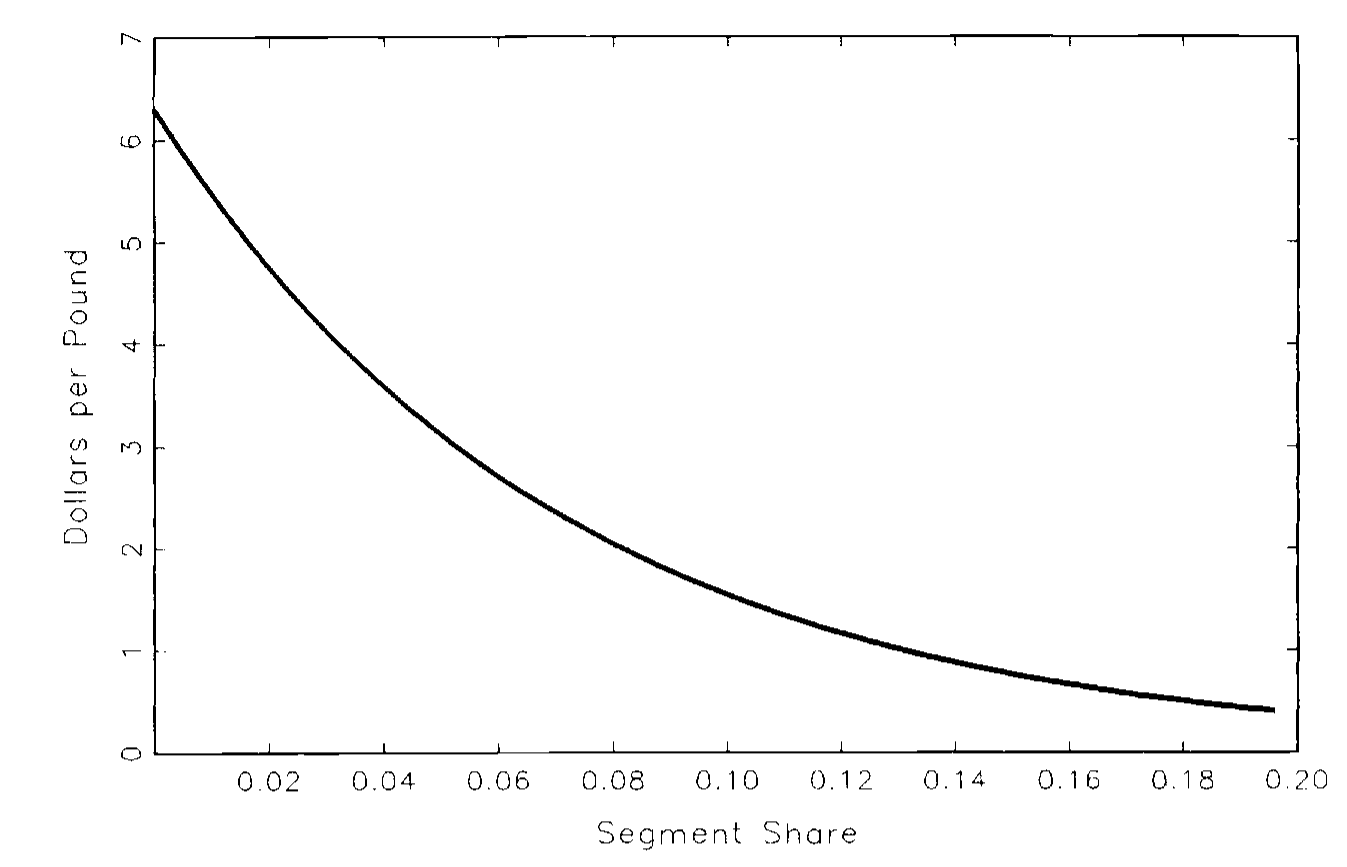
\includegraphics[width=\textwidth]{figures/ch10/hausman_fig5_1.png}
\caption{Method 1: demand at average regressors}
\end{subfigure}\hfill
\begin{subfigure}[t]{0.49\textwidth}
\centering
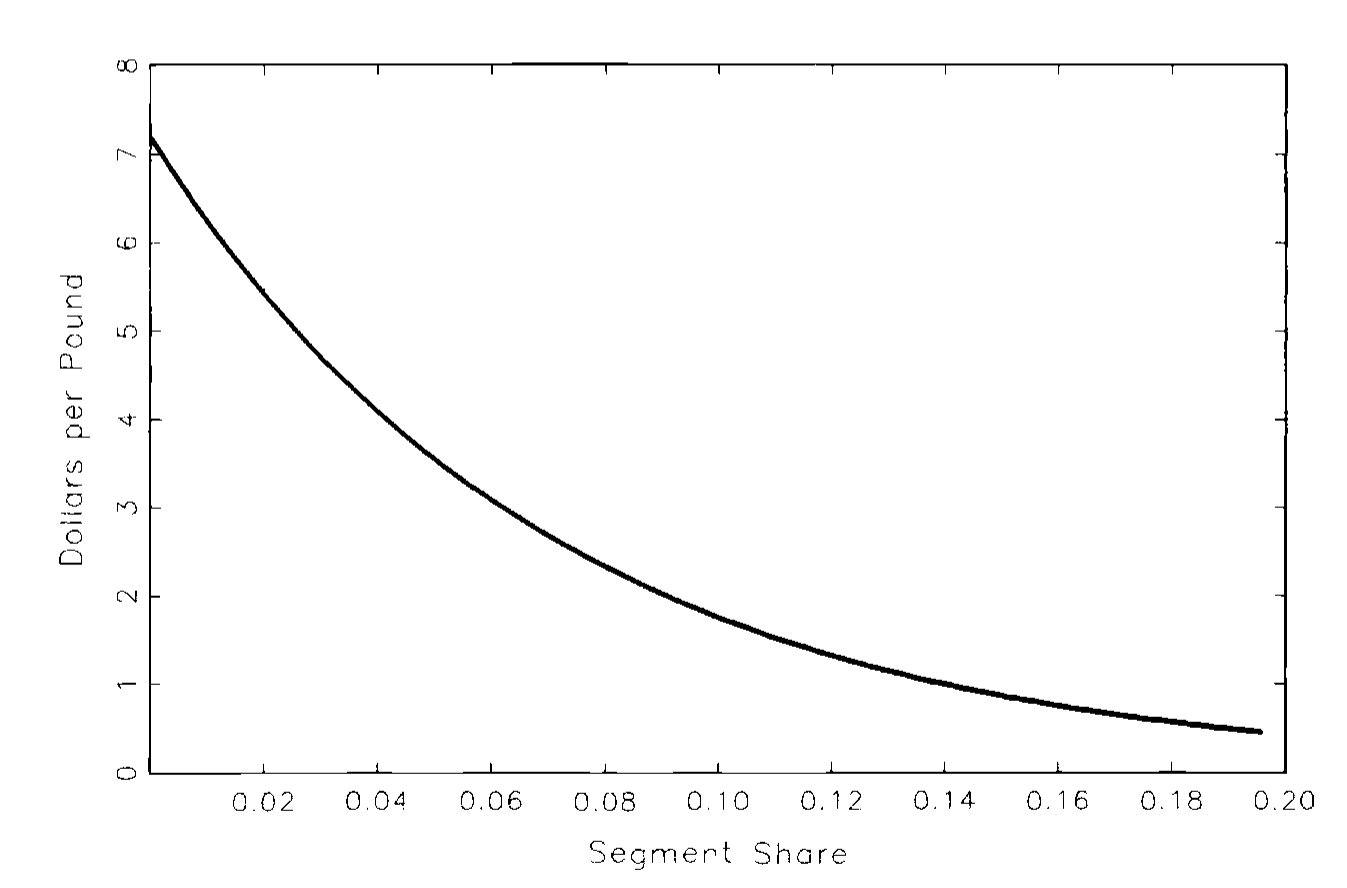
\includegraphics[width=\textwidth]{figures/ch10/hausman_fig5_2.png}
\caption{Method 2: average of 959 city-week curves}
\end{subfigure}
\caption{Estimated AIDS demand curves for Apple-Cinnamon Cheerios. The horizontal axis is ACC's share of
family-segment spending and the vertical axis is the price in dollars per pound. The intercept on the price
axis is the virtual price. Source: Hausman (1997), Figures 5.1 and 5.2.}
\label{fig:10-hausman-aids-curves}
\end{figure}

\casehead{Virtual price}
City virtual prices range from about \$6.00 to about \$7.50. Hausman's best estimate of the aggregate
virtual price is \$7.14, with an asymptotic standard error of \$1.33 (p.~227). The lower end of an
approximate 95 percent confidence interval is \$4.75. Hausman describes it as 35 percent above ACC's average
price of \$3.48 (36.5 percent by our computation).\footnote{A symmetric normal interval would give
$7.14 - 1.96\times 1.33 = \$4.53$ (our computation). Hausman does not say how he computes \$4.75.} The virtual price is about twice the actual price. Hausman finds this reasonable given an own
elasticity of about $-2.2$ (p.~228).

\casehead{Exact consumer surplus}
The exact compensating variation is computed from the expenditure function, by the method of
\citet{HausmanNewey1995} (fn.~24). It is close to the area under the demand curve above \$3.48. The estimate
is \$32,268 per city per week, with an asymptotic standard error of \$3,384 (p.~228). For the United States
it amounts to about \$78.1 million per year, or about \$0.3136 per person per year. Hausman anticipates the
objection that his method yields small elasticities. The same technique gives own-price elasticities for
beer brands between about $-4.0$ and $-6.2$ in \citet{HausmanLeonardZona1994} (fn.~25).

\casehead{A bound robust to extrapolation}
Observed prices never come near the virtual price, so \$7.14 rests on the shape of the estimated curve far
outside the data. Hausman addresses this with a supporting line. If demand is convex, the tangent at the
observed point lies below the curve and meets the price axis below the true intercept. This is the logic of
\cref{prop:10-tangent}. Drawing the tangent to the curves of \cref{fig:10-hausman-aids-curves} at \$3.48
gives lower bounds between \$5.55 and \$5.94, with a standard error of about \$0.15 (p.~228). The bounds lie
about 65 percent above the average price.\footnote{The tangents are drawn in the share-price plane of the
figures. In the quantity-price plane, \cref{prop:10-tangent} with ACC's overall elasticity of $-2.173$ gives
$3.48\bigl(1 + \frac{1}{2.173}\bigr) = \$5.08$ (our computation). Convexity in one plane does not imply
convexity in the other, since the share is proportional to price times quantity.}

\casehead{Two consistency checks}
Two checks of our own relate these numbers to the theory of \cref{sec:10-virtual}. Hausman's pound volumes
and prices imply family-segment spending of about \$1.14 million per city-week, so ACC sells about 20,300
pounds a week in a typical city.\footnote{We compute these figures from Table 5.2 and p.~234. Cheerios sells 93,738
pounds at \$2.644 with a segment share of 0.216, and Honey-Nut sells 47,215 pounds at \$3.605 with a share of
0.150. The two imply segment spending of \$1.147 and \$1.133 million. ACC's volume is
$\frac{0.0619 \times 1.14\text{ million}}{3.48}$.} First, the Paasche rectangle of
\cref{prop:10-index-bounds} is $(7.14 - 3.48)\times 20{,}300 \approx \$74{,}200$. The exact surplus,
\$32,268, is 43 percent of it. A linear Hicksian curve would give exactly half, and a convex curve lies below
the chord, so the share below one half is what convexity predicts. Second, the rectangle is about 1.7 percent
of cereal spending, which matches the index effect Hausman reports below.

\begin{table}[htbp]
\centering
\caption{Welfare effects of Apple-Cinnamon Cheerios}\label{tab:10-hausman-welfare}
\begin{threeparttable}
\begin{tabular}{@{}lll@{}}
\toprule
Quantity & Estimate & Page \\
\midrule
\multicolumn{3}{@{}l}{\textit{Perfect competition (AIDS)}} \\
Virtual price, aggregate & \$7.14 (1.33) & 227 \\
Virtual price, range across cities & \$6.00 to \$7.50 & 227 \\
Lower end of approximate 95\% interval & \$4.75 & 227 \\
Tangent lower bound on virtual price & \$5.55 to \$5.94 (about 0.15) & 228 \\
Consumer surplus per city per week & \$32,268 (3,384) & 228 \\
Consumer surplus, United States, per year & \$78.1 million & 228 \\
Consumer surplus per person per year & \$0.3136 & 228 \\[2pt]
\multicolumn{3}{@{}l}{\textit{Alternative specification}} \\
CES virtual price & infinite & 231 \\
CES consumer surplus & about $3 \times$ AIDS & 231 \\[2pt]
\multicolumn{3}{@{}l}{\textit{Imperfect competition (rivals' prices fixed)}} \\
Loss from higher Cheerios prices, city-week & \$890 + \$3,715 = \$4,605 & 234 \\
Net gain per city-week & \$27,395 (85.6\% of \$32,000) & 234 \\
Net gain, United States, per year & \$66.8 million, \$0.268 per person & 234 \\[2pt]
\multicolumn{3}{@{}l}{\textit{Cereal price index}} \\
Overstatement, perfect competition & about 25\% & 229 \\
Overstatement, imperfect competition & about 20\% & 234 \\
\bottomrule
\end{tabular}
\begin{tablenotes}[flushleft]\footnotesize
\item Notes: Compiled from the text of \citet{Hausman1997}, pp.~227--234. Asymptotic standard errors in
parentheses. The net gain uses a rounded perfect-competition surplus of \$32,000. The index overstatements
refer to the cumulative effect of brands introduced over ten years.
\end{tablenotes}
\end{threeparttable}
\end{table}

\Cref{tab:10-hausman-welfare} collects the welfare results of the paper.

\subsection{Implications for the cereal price index}\label{sec:10-hausman-index}

Hausman translates the surplus into a price-index correction (pp.~228--229). Treating ACC as part of
Honey-Nut Cheerios would show almost no effect, beyond ACC's slightly lower price. Suppose instead, contrary
to fact, that all of ACC's share came from Honey-Nut. With ACC valued at its virtual price before
the introduction, the price index of the two brands falls from about \$4.60 to about \$3.57, or 22 percent. The
family-segment index falls from \$3.10 to \$2.88, or 7.1 percent. The overall cereal index falls by about
0.017, or \$0.052, about 1.7 percent. These figures are share-weighted average prices with ACC valued at
\$7.14 in the base period.\footnote{We approximately reproduce these figures from Table 5.2. The Honey-Nut and
ACC composite is $\frac{15.03 \times 3.605 + 6.19 \times 7.14}{21.22} = \$4.64$ before and
$\frac{15.03 \times 3.605 + 6.19 \times 3.48}{21.22} = \$3.57$ after, a fall of 23 percent. The family index is
\$2.88 with ACC at \$3.48 and \$3.11 with ACC at \$7.14. The small gaps from Hausman's \$4.60, 22 percent and
\$3.10 presumably reflect rounding.}

Hausman then states a rule of thumb. The change in the overall index is approximately ACC's share of cereal
spending, 1.6 percent, times the gap between the virtual and the actual price relative to the actual price.
If the virtual price is twice the actual price, the index change roughly equals the new brand's share. About
25 percent of cereal demand comes from brands introduced in the previous ten years. Suppose these brands sell
at about the same prices as old ones and have virtual prices twice their actual prices. Then the cereal index
that ignores them is too high by about their share, 25 percent (p.~229). Exits reduce the gain, but brands
are withdrawn only when their shares are tiny, so the correction is small and could not be estimated
(fn.~26).

The rule of thumb is the Paasche rectangle of \cref{prop:10-index-bounds}, expressed as a share of spending:
$w_n\bigl(\frac{p_n^V}{p_n} - 1\bigr)$. The proposition shows that this rectangle exceeds the exact gain for
any downward-sloping Hicksian curve. Hausman's own surplus estimate is 43 percent of the rectangle, about
0.75 percent of cereal spending against the 1.7 percent of the rule. Applying the same ratio to his
extrapolation would cut the 25 percent figure to about 11 percent, and the imperfect-competition figure of
20 percent to about 9 percent.\footnote{We compute $0.435 \times 25 = 10.9$ and
$0.435 \times 0.856 \times 25 = 9.3$. The extrapolation also assumes that every new brand of the decade
resembles ACC, a strong assumption that Hausman calls ``perhaps unrealistic'' (p.~229).} The correction
remains large by the standards of price measurement. The main conclusion survives, but the rectangle
overstates the exact effect by a factor of about two.

\subsection{Alternative specifications: attributes, logit and CES}\label{sec:10-hausman-ces}

Section 5.5 of the paper explains why Hausman prefers a flexible product-space system. Attribute models in
the Hotelling, Gorman and Lancaster tradition describe a product by its characteristics and predict demand
for new products from them (\citealp[fn.~27]{Hausman1997}, citing \citealp{PakesBerryLevinsohn1993}).
Hausman argues that ACC cannot be described by attributes, ``perhaps the volume of apples and cinnamon''
(p.~229). He adds that no metric measures how close attributes are and no aggregator combines them. The
right measure of closeness, in his view, is the cross-price elasticity. His experience with probit models of
French champagne makes the point: ``the bubble content could never be made to come in significant'' (fn.~28,
on the models of \citealp{HausmanWise1978}). The logit model has the independence of irrelevant alternatives
(IIA) property, which ``typically leads to a vast overestimate'' of the surplus from a new good (p.~230). The
nested logit still has IIA within each nest. \Cref{sec:10-charspace} takes up the case for characteristics
models.

\casehead{CES demand}
Hausman compares his estimates with the constant elasticity of substitution (CES) model of
\citet{DixitStiglitz1977}, which treats all goods symmetrically. Utility is
\begin{equation}\label{eq:10-h-ces-u}
  U(x_1,\dots,x_n) = \Bigl(\sum_{i=1}^{n}x_i^{\rho}\Bigr)^{\frac{1}{\rho}}, \qquad 0 < \rho < 1
\end{equation}
(Hausman's eq.~9). Write $\eta = \frac{1}{1-\rho}$ for the elasticity of substitution, so that
$1 - \eta = -\frac{\rho}{1-\rho}$. Maximizing \eqref{eq:10-h-ces-u} subject to $\sum_i p_ix_i = y$ gives the
Marshallian demand implied by \eqref{eq:10-ces-share} with equal taste parameters,
\begin{equation}\label{eq:10-h-ces-demand}
  x_k = \frac{y\,p_k^{-\eta}}{\sum_{i=1}^{n}p_i^{1-\eta}}.
\end{equation}
Hausman's eq.~10 writes the compensated version. The unit expenditure function is
$c(p) = \bigl(\sum_ip_i^{1-\eta}\bigr)^{\frac{1}{1-\eta}}$, and Hicksian demand is
$x_k = U\bigl(\frac{p_k}{c(p)}\bigr)^{-\eta} = U\,p_k^{-\eta}\bigl(\sum_ip_i^{1-\eta}\bigr)^{-\frac{\eta}{\eta-1}}$.
Since $\frac{\eta}{\eta-1} = \frac{1}{\rho}$, this equals
$\bigl[\frac{\sum_ix_i^{\rho}}{\sum_ip_i^{-\frac{\rho}{1-\rho}}}\bigr]^{\frac{1}{\rho}}p_k^{-\frac{1}{1-\rho}}$, which
is eq.~10 without its error term. Taking logs of \eqref{eq:10-h-ces-demand},
$\ln x_k = \ln y - \eta\ln p_k - \ln\sum_ip_i^{1-\eta}$. Differentiating with respect to $\ln p_j$ and writing
$w_j = \frac{p_j^{1-\eta}}{\sum_ip_i^{1-\eta}}$ for the spending share,
\begin{equation}\label{eq:10-h-ces-elast}
  \varepsilon_{kj} = -\eta\,\indic\{k = j\} + (\eta - 1)w_j.
\end{equation}
Every product has the same cross elasticity with respect to $p_j$, which is Hausman's eq.~11. Own elasticities
depend only on the share and on $\eta$, ``a property without any empirical foundation'' (p.~231). Demand
\eqref{eq:10-h-ces-demand} is positive at every finite price, so the CES virtual price is infinite.

\casehead{Estimates}
Hausman estimates the CES model by nonlinear two-stage least squares (p.~231). He reports
$\hat\rho = 0.580$ with an asymptotic standard error of 0.00001 and an elasticity of substitution of 2.13.
The two printed numbers are inconsistent, since $\frac{1}{1 - 0.580} = 2.38$, while 2.13 corresponds to
$\rho = 0.53$. We cannot tell which is the typographical error. \Cref{fig:10-hausman-ces} shows the
estimated CES curve. It rises steeply as the share approaches zero and never meets the price axis. The
consumer surplus, the area under this curve above the price, is ``about three times as high'' as the AIDS
estimate of \$78.1 million a year (p.~231).

\begin{figure}[htbp]
\centering
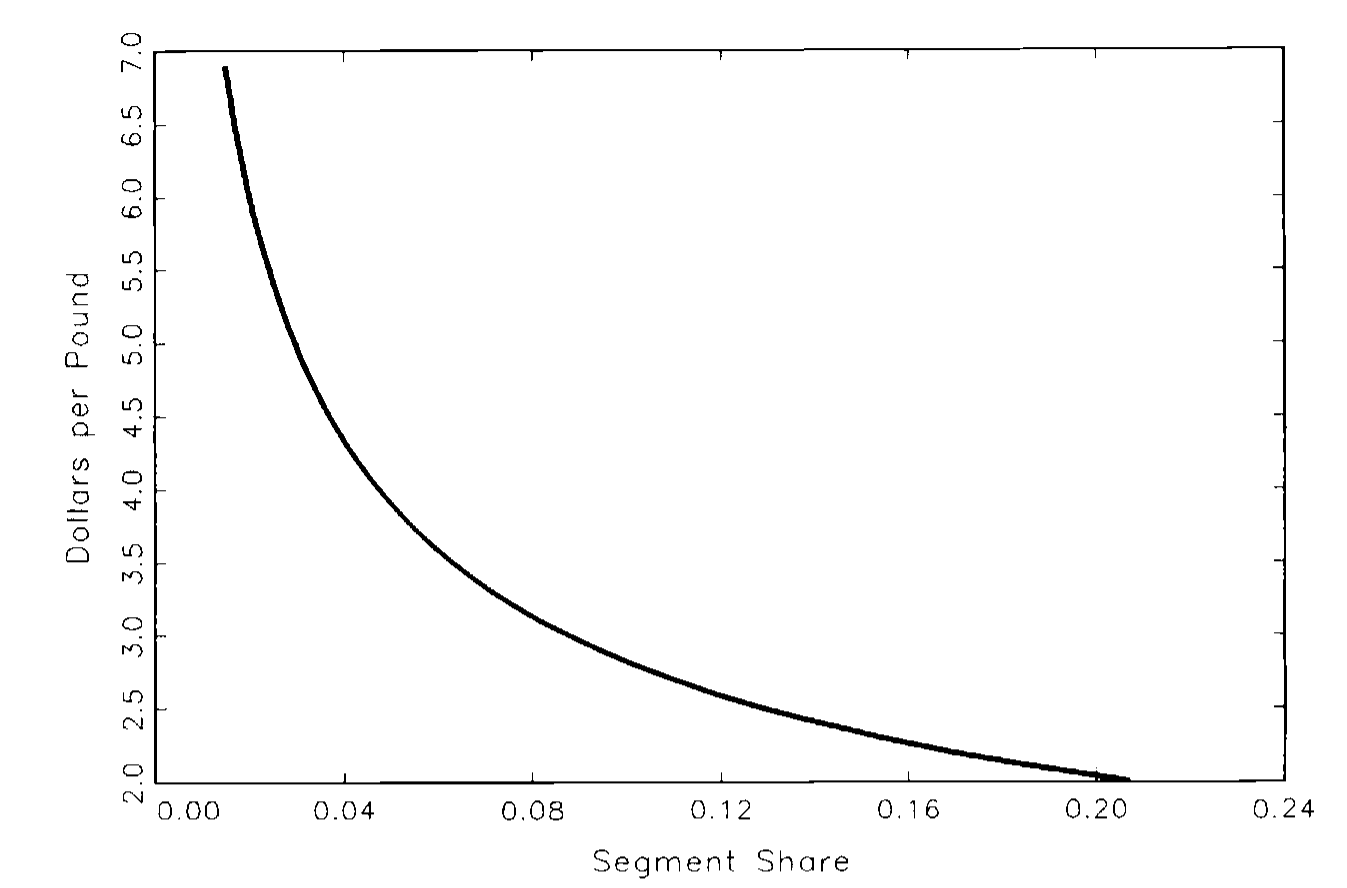
\includegraphics[width=0.75\textwidth]{figures/ch10/hausman_fig5_3.png}
\caption{Estimated CES demand curve for family-segment brands. The horizontal axis is the segment share and
the vertical axis the price in dollars per pound. The curve never meets the price axis, so the virtual price
is infinite. Source: Hausman (1997), Figure 5.3.}
\label{fig:10-hausman-ces}
\end{figure}

The comparison teaches a lesson about functional form. At ACC's segment share of 0.0619,
\eqref{eq:10-h-ces-elast} gives an own elasticity of $-2.13 + 1.13 \times 0.0619 = -2.06$ with $\eta = 2.13$.
This is close to the AIDS value of $-2.12$. The two systems thus give similar own elasticities at the data and diverge
mainly in the extrapolation to zero quantity. The share-only CES formula of \cref{cor:10-ces-newgood} implies,
as computed in \cref{sec:10-feenstra}, that ACC lowers the cost of living of the family segment by 5.5 percent.
The equivalent variation is then 5.5 percent of family-segment spending, about \$63,000 per city-week, and the
compensating variation is 5.8 percent. Both are about twice the AIDS surplus. With $\eta = 2.38$ the fall in the
cost of living is 4.5 percent.\footnote{These are our computations,
using segment spending of \$1.14 million per city-week. Hausman's ``three times'' integrates his estimated
CES curve, so the two comparisons are not identical. Both put the CES valuation at a multiple of the AIDS
valuation.} In the CES and the logit, the value of variety is built into the functional form. The AIDS
lets the data choose a finite virtual price, at the cost of relying on the curvature of the estimated curve.

\subsection{Imperfect competition}\label{sec:10-hausman-imperfect}

The classical analysis assumes that other prices stay at marginal cost when the new good arrives. Hausman
notes that most new brands come from multiproduct firms (p.~231). When General Mills raises the price of
Cheerios, some of the lost buyers now switch to ACC instead of a rival brand. The firm keeps that demand, so
the introduction lets it raise the prices of its existing brands. This effect lowers the consumer gain.

\casehead{Pricing equations}
\Cref{sec:10-multiproduct} derives Hausman's pricing equations in the notation of this chapter. A single-product
firm under Nash-Bertrand pricing sets $\frac{p_1 - mc_1}{p_1} = -\frac{1}{\varepsilon_{11}}$ (Hausman's eq.~12). A
firm selling brands $k = 1,\dots,K$ satisfies the elasticity form \eqref{eq:10-foc-elast} of its first-order
conditions (his eq.~13), with $w_k$ the revenue share of brand $k$ in the firm's sales. In matrix form these are
\eqref{eq:10-foc-matrix}, $w + E^\top m = 0$ and $m = -(E^\top)^{-1}w$ (his eqs.~14 and 15), where
$m_k = \frac{p_k - mc_k}{p_k}w_k$. Dividing each $m_k$ by $w_k$ gives the Lerner index of brand $k$.

\casehead{The calculation}
Hausman solves \eqref{eq:10-foc-matrix} for the General Mills family brands with ACC and without it. He
holds marginal costs constant and assumes that ``other firms, such as Kellogg, will not change their prices
in response to the introduction'' (p.~234). He claims that the resulting price changes are ``a lower bound
on expected price changes, absent new entry by competitors'' (p.~233). \Cref{tab:10-hausman-margins}
reproduces the results.

\begin{table}[htbp]
\centering
\caption{Nash-Bertrand price-cost margins of the General Mills family brands}\label{tab:10-hausman-margins}
\begin{threeparttable}
\begin{tabular}{@{}lcc@{}}
\toprule
 & Cheerios & Honey-Nut Cheerios \\
\midrule
Price-cost margin & 0.5268 & 0.5203 \\
Price-cost margin without Apple-Cinnamon Cheerios & 0.5251 & 0.5096 \\
Price-cost margin if brand were independent & 0.5193 & 0.5050 \\
\bottomrule
\end{tabular}
\begin{tablenotes}[flushleft]\footnotesize
\item Notes: Reproduced in full from \citet[Table 5.7]{Hausman1997}. Margins are Lerner indexes
$\frac{p - mc}{p}$ from \eqref{eq:10-foc-matrix}. The last row is $-\frac{1}{\varepsilon_{jj}}$ with the overall
own elasticities of Table 5.6: $\frac{1}{1.92572} = 0.5193$ and $\frac{1}{1.98037} = 0.5050$. Rivals' prices
and marginal costs are held fixed.
\end{tablenotes}
\end{threeparttable}
\end{table}

The margins rise when ACC joins the line, and they exceed the single-product margins of the last row. With
constant marginal cost, \eqref{eq:10-price-ratio} converts the margins into the ratio
$r_k = \frac{p_k^{\text{with}}}{p_k^{\text{without}}}$ of the prices with and without ACC. The 1992 prices of
Table 5.2 are observed with ACC on the market. The price without ACC is therefore $\frac{p_k^{\text{with}}}{r_k}$,
and the price increase is $p_k^{\text{with}} - \frac{p_k^{\text{with}}}{r_k} = p_k^{\text{with}}\bigl(1 - \frac{1}{r_k}\bigr)$.
For Cheerios, the ratio is $\frac{1 - 0.5251}{1 - 0.5268} = \frac{0.4749}{0.4732} = 1.0036$. At the 1992 price of \$2.644
the increase is $2.644 \times \bigl(1 - \frac{0.4732}{0.4749}\bigr) = \$0.0095$. For Honey-Nut, the ratio is
$\frac{0.4904}{0.4797} = 1.0223$, and at \$3.605 the increase is
$3.605 \times \bigl(1 - \frac{0.4797}{0.4904}\bigr) = \$0.0787$. Both are the figures Hausman
reports.\footnote{This is our computation. The implied prices without ACC are \$2.635 and \$3.526. The paper
also reports markup increases of 0.32 and 3.0 percent. The first is the ratio of the Cheerios
margins, $\frac{0.5268}{0.5251} = 1.0032$. The same ratio for Honey-Nut is 1.021.} The larger effect on
Honey-Nut is expected, since ACC is a closer substitute for Honey-Nut than for Cheerios.

\casehead{Welfare}
Average weekly sales per city are 93,738 pounds of Cheerios and 47,215 pounds of Honey-Nut (p.~234). To first
order, the price increases cost consumers $0.0095 \times 93{,}738 = \$890$ and $0.0787 \times 47{,}215 =
\$3{,}715$ per city-week, a total of \$4,605. Hausman compares this loss with ``the \$32,000--44,000 consumer's
surplus estimates''. The net gain is $\$32{,}000 - \$4{,}605 = \$27{,}395$, which is 85.6 percent of the
Hicksian gain (p.~234). Per year the gain is \$66.8 million, or \$0.268 per person. The overstatement of the
cereal CPI falls from about 25 percent to about 20 percent. Hausman notes that his data begin after ACC's
launch, so he cannot compare prices before and after it directly. He leaves such a study for future research
(p.~234).

\casehead{What the calculation holds fixed}
Reproducing Table 5.7 shows exactly what the counterfactual changes. The ``without'' row deletes ACC's row and
column from the elasticity matrix and ACC's entry from the share vector. It keeps the shares and elasticities
of Cheerios and Honey-Nut at their values with ACC present.\footnote{This is our computation. We solve
\eqref{eq:10-foc-matrix} with the mean revenue shares of Table 5.5 and the Cheerios block of Table 5.6. The
solution reproduces the four margins in the first two rows of Table 5.7 to four decimals.} In the language of
\cref{sec:10-imperfect}, the calculation captures only the new term that ACC adds to the first-order
conditions. Before the launch, Cheerios and Honey-Nut had larger shares. The fall in their shares is the
source of the two offsetting effects that \citet{Bresnahan1997} stresses, and the calculation omits it.
Rivals' prices are held fixed as well. \Cref{sec:10-bresnahan-competition}
returns to both points.

\begin{remark}[The orientation of the elasticity matrix in Table 5.7]\label{rem:10-margins-orientation}
Table 5.7 is reproduced exactly when Table 5.6 is read with rows as quantities, the layout that
\eqref{eq:10-foc-matrix} requires. \Cref{rem:10-orientation} shows that Table 5.6 is printed with rows as
prices. The two facts together imply that the margins were computed with $\varepsilon_{jk}$ where
\eqref{eq:10-foc-elast} requires $\varepsilon_{kj}$. Recomputing with the layout implied by
\cref{rem:10-orientation}, and changing nothing else, gives margins with ACC of 0.5250 (Cheerios), 0.5402
(Honey-Nut) and 0.5251 (ACC), and without ACC of 0.5215 and 0.5169. Relative to the prices without ACC,
the implied increases are 0.7 percent for Cheerios and 5.1 percent for Honey-Nut. In dollars,
$p_k^{\text{with}}\bigl(1 - \frac{1}{r_k}\bigr)$ gives \$0.0192 and \$0.1739 per pound. The first-order loss becomes
\$10,004 per city-week, and the net gain 68.7 percent of \$32,000.\footnote{We computed these values with
\texttt{figures/ch10/src/hausman\_reproduction.py}. With the printed layout, the same program gives ACC's own
margin as 0.6201, a value the paper does not report.} The direction is intuitive. In Honey-Nut's first-order
condition the relevant cross effect is the response of ACC's volume to Honey-Nut's price, which is 0.21. The
printed layout uses instead the response of Honey-Nut's volume to ACC's price, which is 0.08. We offer this
as a reproduction exercise, since the paper itself does not confirm our reading of Table 5.6. It shows that
the imperfect-competition adjustment is sensitive to a detail that papers rarely state, the layout of the
elasticity matrix.
\end{remark}

\subsection{Robustness}\label{sec:10-hausman-robustness}

The paper reports several robustness checks, mostly in footnotes. Monthly data give elasticities similar to
the weekly estimates, with less precision (fn.~21). The segmentation is not rejected by specification tests
(fn.~22). A middle level that does not impose exact two-stage budgeting gives similar results (fn.~17). The
choice between exact and Stone segment indexes ``does not typically have much influence'' (p.~218). The two
aggregation methods for the virtual price give intercepts of about \$6.30 and \$7.20. The tangent bound
limits the role of extrapolation, and the CES comparison shows the direction of functional-form bias.

Other checks are missing. The paper reports no estimates with alternative instruments, no first-stage
statistics and no outcome of the overidentification tests that fn.~20 mentions. It reports no test of the
independence of demand shocks across cities, the assumption on which identification rests. Table 5.7 has no
standard errors, and the imperfect-competition calculation fixes rivals' prices without a sensitivity
analysis. \Cref{sec:10-bresnahan} shows why the first omission matters most.

\subsection{Interpretation, critiques and contribution}\label{sec:10-hausman-assessment}

Taken at face value, the estimates say that consumers value even a close variant of existing brands
highly. ACC's demand curve is steep relative to its volume. The virtual price is twice the actual price, and
the surplus is about 46 percent of ACC's revenue.\footnote{By our computation, the surplus of \$32,268 compares with revenue of
about \$70,600 per city-week.} If incremental brands are typical, official price indexes for branded
consumer goods understate real income growth.

Four lines of critique follow from the theory of this chapter. First, the estimates rest on instruments that
fail if national demand shocks move prices in all cities at once (\cref{sec:10-bresnahan-iv}). Second, the
virtual price is an extrapolation, and the surplus depends on the curvature of the AIDS curve beyond the data
(\cref{sec:10-functional}). The tangent bound helps, but it requires convexity. Third, the
imperfect-competition adjustment holds rivals' prices fixed and keeps post-launch shares in the
counterfactual (\cref{sec:10-bresnahan-competition}). Fourth, the price-index extrapolation uses the Paasche
rectangle, which exceeds the exact gain, and assumes that all new brands resemble ACC
(\cref{sec:10-hausman-index}).

The paper made several contributions. It showed how to compute the exact value of a new brand from scanner
data. It combined the virtual price of \citet{Hicks1940} and \citet{Rothbarth1941} with the exact surplus
methods of \citet{Hausman1981} and \citet{HausmanNewey1995}. Together with \citet{HausmanLeonardZona1994}, it
made multistage budgeting with an unrestricted bottom level a practical tool. The two papers also introduced
prices in other markets as instruments, now a standard device in demand estimation \citep{Nevo2001}. Finally, it raised the question of how market power changes the value of
a new good. The answer it gave was incomplete, as the next section explains, but the question has shaped the
literature since, including the work of \citet{Petrin2002} in \cref{sec:10-petrin}.

\section{Bresnahan's Comment: instruments and competition}\label{sec:10-bresnahan}

\citet{Bresnahan1997} accepts the importance of the question and much of the specification. He disputes
the instruments and the treatment of competition. His comment opens with a statistic: \emph{Brandweek}
counted over 22,000 new-product introductions in 1994 (p.~237). Theory cannot say whether markets supply too
many or too few varieties (fn.~1, quoting \citealp{EatonLipsey1989}, as discussed in \cref{sec:10-private-social}).
So the value of incremental variety is an empirical question, and Hausman's paper is an important attempt to
answer it. This section develops Bresnahan's four points in turn, with the formal
analysis that he sketches in his appendix.

\subsection{Why a steep single-product demand curve means large value}\label{sec:10-bresnahan-dd}

Bresnahan frames the issue with \cref{fig:10-dd-DD}. The steep curve $DD$ is market demand. The flatter
curve $dd$ is the demand for one product when the prices of its substitutes are held fixed. The flat line
$dd(-\infty)$ is the demand for a product that is a perfect substitute for others. Introducing a product at
price $P_1$ creates the shaded triangle between $dd$, the price axis and the line at $P_1$. Before the
introduction the product was in effect priced at $P_0$, where $dd$ meets the price axis. This is the virtual
price of \cref{sec:10-virtual}.

\begin{figure}[htbp]
\centering
\begin{tikzpicture}[scale=1.0, >=Stealth]
  \draw[->] (0,0) -- (7.4,0) node[below] {$Q$};
  \draw[->] (0,0) -- (0,5.4) node[left] {$P$};
  \fill[black!70] (0,4) -- (0,2.9) -- (2.383,2.9) -- cycle;
  \draw[thick] (1.6,5.0) -- (5.3,0.17) node[right] {$DD$};
  \node at (1.95,5.15) {$DD$};
  \draw[thick] (0,4) -- (6.8,0.862) node[right] {$dd$};
  \node at (0.95,3.8) {$dd$};
  \draw[thick] (0,2.311) -- (7.0,2.311) node[right] {$dd(-\infty)$};
  \draw[dashed] (2.383,2.9) -- (2.383,0);
  \node[left] at (0,4) {$P_0$};
  \node[left] at (0,2.9) {$P_1$};
  \node[below] at (2.383,0) {$q_1$};
  \fill (3.659,2.311) circle (1.5pt);
\end{tikzpicture}
\caption{Consumers' gain from a new product. $DD$ is market demand, $dd$ the demand for a single product at
fixed prices of its substitutes, and $dd(-\infty)$ the demand for a perfect substitute. Selling the product
at $P_1$ instead of its choke price $P_0$ yields the shaded surplus. The steeper is $dd$, the larger the
triangle for a given volume $q_1$. Source: redrawn after Bresnahan (1997), Figure 5C.1.}
\label{fig:10-dd-DD}
\end{figure}

The area of the triangle makes the point precise. Let $dd$ be linear with slope $-s$ in the $(Q, P)$ plane,
where $s > 0$ measures its steepness. A product sold at $P_1$ in volume $q_1$ then has choke price
$P_0 = P_1 + s\,q_1$. Its surplus is
\begin{equation}\label{eq:10-b-triangle}
  CS = \frac{1}{2}(P_0 - P_1)\,q_1 = \frac{s}{2}\,q_1^2.
\end{equation}
For a given volume the surplus is proportional to the steepness $s$, and it vanishes as $dd$ flattens to
$dd(-\infty)$. Treating new goods as perfect substitutes, as hedonic quality adjustment implicitly does,
therefore sets their value to zero. Linking a new good into a price index late treats it as irrelevant in
its early life, and the later the link, the larger the error (p.~238). Both practices understate the value
of new goods. Bresnahan notes a converse in fn.~2. If a new good is a perfect substitute, the law of one price
holds, and late linking does no harm.

Hausman's finding is a steep $dd$ for ACC. \citet{Trajtenberg1989}, whose work \cref{sec:10-trajtenberg}
studies, conjectured that the distance of a new good from existing products in characteristics space governs
the slope of $dd$ (fn.~3). The same steepness has a second implication, developed in
\cref{sec:10-bresnahan-competition}. A product with a steep $dd$ that is sold by one firm carries market
power. Consumer surplus and imperfect competition are therefore linked from the start.

\subsection{Is the large surplus an artifact of the specification?}\label{sec:10-bresnahan-spec}

Bresnahan concludes that it is not (pp.~239--240). A skeptic might suspect that existing Cheerios products
already satisfy ``pretty much any palate''. Hausman's large surplus must then come from finding poor
substitutability between ACC and the other family brands. Within the segment, the AIDS imposes almost no
structure on own and cross elasticities, so the finding comes from the data. The more restrictive CES gives
an even larger surplus (fn.~4).

The segment structure is an assumption, which Bresnahan does not find worrying. It is not interesting to
ask whether two children's cereals substitute more closely than a children's cereal and Special K. The
segments come from marketing research based on richer data, including consumer microdata. Bresnahan adds a
caution for other industries (fn.~5). In automobiles, brand names and country reputations compete with size
classes as principles of grouping, and in many consumer goods private labels form a further group. The
simple structure of cereal is the exception.

\subsection{Instruments and national demand shocks}\label{sec:10-bresnahan-iv}

The treatment of price endogeneity is the other place where the conclusion might have been ``accidentally
assumed'' (p.~240). Hausman's identifying assumption is that the shocks $\omega_{jnt}$ in
\eqref{eq:10-h-price} are independent across cities. This rules out every national shock to the demand for
one brand relative to another. In Bresnahan's words, ``there can be no successful nationwide advertising
campaigns which shift the demand for individual brands or products'' (p.~241). There can be no national
fads and no slow national acceptance of new brands. Including advertising in the demand system does not
solve the problem, because the econometrician does not observe which campaigns succeed (fn.~6).

Hausman's fallback is that prices are predetermined. Economically, this requires that national demand shocks
cannot be foreseen when prices are set. Bresnahan finds this unlikely for shocks such as advertising
campaigns, which manufacturers plan and communicate to retailers in advance. If national shocks exist and
are reflected in prices, and if supply slopes up, prices in other cities are correlated with the demand
error. Supply slopes up in the one-week run because inventories cannot adjust or because of market power
(fn.~7). Hausman's own pricing equations imply an upward-sloping supply relation.

\casehead{The model}
We formalize the argument with one product, following Bresnahan's simple case: linear demand, single-product
Bertrand pricing and constant marginal cost (p.~241). In city $n$ and week $t$,
\begin{equation}\label{eq:10-b-demand}
  q_{nt} = d_n - b\,p_{nt} + \xi_{nt}, \qquad b > 0,
\end{equation}
where $d_n$ is a city effect. Marginal cost is $c_{nt} = c_n + k_t + v_{nt}$. The national cost component
$k_t$ has variance $\sigma_k^2$, and the local component $v_{nt}$ has variance $\sigma_v^2$. The demand error
has a national and a local part, $\xi_{nt} = \chi_t + e_{nt}$. Each part splits into a component that is
anticipated when prices are set and one that is not: $\chi_t = \chi^a_t + \chi^u_t$ and
$e_{nt} = e^a_{nt} + e^u_{nt}$, with variances $\sigma_{\chi a}^2$, $\sigma_{\chi u}^2$, $\sigma_{ea}^2$ and
$\sigma_{eu}^2$. All components have mean zero and are mutually independent. Local components are
independent across cities. City effects are removed by the within transformation, so we treat $d_n$ and
$c_n$ as known.

\casehead{Pricing}
The firm sets $p_{nt}$ to maximize expected profit $\E[(p - c_{nt})(d_n - bp + \xi_{nt})\mid\mathcal{I}_{nt}]$,
where the information set $\mathcal{I}_{nt}$ contains costs and the anticipated shocks. The first-order
condition is
\begin{equation*}
  d_n - 2b\,p_{nt} + \E[\xi_{nt}\mid\mathcal{I}_{nt}] + b\,c_{nt} = 0.
\end{equation*}
Solving for the price,
\begin{equation}\label{eq:10-b-price}
  p_{nt} = \frac{1}{2}\Bigl(c_{nt} + \frac{d_n + \chi^a_t + e^a_{nt}}{b}\Bigr).
\end{equation}
Equivalently $p_{nt} = c_{nt} + \frac{\E[q_{nt}\mid\mathcal{I}_{nt}]}{b}$, the expected-quantity version of
Bresnahan's supply relation $P = Q(-\gamma_{jj})^{-1} + c$. With fully anticipated shocks this is his model,
and with no anticipated shocks prices are predetermined in Hausman's sense.

\casehead{Estimators}
The Hausman estimator of $-b$ is the instrumental-variables (IV) estimator that uses $p_{\ell t}$, the
price in another city $\ell\neq n$, as the instrument for $p_{nt}$. Averaging over several other cities, as
our simulation does, has the same probability limit. Ordinary least squares (OLS) regresses $q_{nt}$ on
$p_{nt}$. Both use within-city deviations.

\begin{proposition}[Hausman instruments with national demand shocks]\label{prop:10-hausman-iv-bias}
In the model given by \eqref{eq:10-b-demand} and \eqref{eq:10-b-price}, define
\begin{equation*}
  \lambda = \frac{\sigma_{\chi a}^2}{b^2\sigma_k^2 + \sigma_{\chi a}^2}, \qquad
  \lambda_{OLS} = \frac{\sigma_{\chi a}^2 + \sigma_{ea}^2}{b^2(\sigma_k^2 + \sigma_v^2) + \sigma_{\chi a}^2 + \sigma_{ea}^2}.
\end{equation*}
Then, as the number of weeks grows,
\begin{equation}\label{eq:10-b-plim}
  \plim\hat b_{IV} = b(1 - 2\lambda), \qquad \plim\hat b_{OLS} = b(1 - 2\lambda_{OLS}).
\end{equation}
Consequently, the following hold.
\begin{enumerate}[label=(\alph*)]
\item The IV estimator is consistent if and only if there are no anticipated national demand shocks,
$\sigma_{\chi a}^2 = 0$. Local shocks, anticipated or not, cause no bias.
\item If $\sigma_{\chi a}^2 > 0$, the estimated demand curve is too steep. If $\sigma_{\chi a}^2 > b^2\sigma_k^2$,
the estimated slope has the wrong sign.
\item Let $\lambda < \frac{1}{2}$, and take linear demand through the observed point $(p, q)$. The implied consumer surplus
$\frac{q^2}{2\hat b}$ and the implied gap $\frac{q}{\hat b}$ between the virtual and the actual price are
both overstated by the factor $\frac{1}{1 - 2\lambda}$.
\item The IV estimator is less biased than OLS if and only if $\lambda < \lambda_{OLS}$.
\end{enumerate}
\end{proposition}

\begin{proof}
Work with within-city deviations, so that $d_n$ and $c_n$ drop out. From \eqref{eq:10-b-price}, the deviation
of the price is
\begin{equation*}
  \tilde p_{nt} = \frac{1}{2}\Bigl(k_t + v_{nt} + \frac{\chi^a_t + e^a_{nt}}{b}\Bigr).
\end{equation*}
Substituting into \eqref{eq:10-b-demand}, the IV and OLS estimators of the coefficient $-b$ converge to
\begin{equation*}
  -b + \frac{\Cov(\tilde p_{\ell t},\xi_{nt})}{\Cov(\tilde p_{\ell t},\tilde p_{nt})}
  \qquad\text{and}\qquad
  -b + \frac{\Cov(\tilde p_{nt},\xi_{nt})}{\Var(\tilde p_{nt})}.
\end{equation*}
For the IV estimator take $\ell\neq n$. The price in city $\ell$ shares only the national components $k_t$ and
$\chi^a_t$ with city $n$. Of these, only $\chi^a_t$ is correlated with $\xi_{nt}$. Hence
\begin{equation*}
  \Cov(\tilde p_{\ell t},\xi_{nt}) = \frac{1}{2b}\Cov(\chi^a_t,\chi_t) = \frac{\sigma_{\chi a}^2}{2b},
\end{equation*}
\begin{equation*}
  \Cov(\tilde p_{\ell t},\tilde p_{nt}) = \frac{1}{4}\Bigl(\sigma_k^2 + \frac{\sigma_{\chi a}^2}{b^2}\Bigr)
  = \frac{b^2\sigma_k^2 + \sigma_{\chi a}^2}{4b^2}.
\end{equation*}
The ratio of the two is
\begin{equation*}
  \frac{\sigma_{\chi a}^2}{2b}\cdot\frac{4b^2}{b^2\sigma_k^2 + \sigma_{\chi a}^2} = 2b\lambda.
\end{equation*}
So the IV estimate of $-b$ converges to $-b + 2b\lambda$, and $\plim\hat b_{IV} = b - 2b\lambda = b(1 - 2\lambda)$.
For OLS the same steps apply with all anticipated components:
\begin{equation*}
  \Cov(\tilde p_{nt},\xi_{nt}) = \frac{\sigma_{\chi a}^2 + \sigma_{ea}^2}{2b}, \qquad
  \Var(\tilde p_{nt}) = \frac{b^2(\sigma_k^2 + \sigma_v^2) + \sigma_{\chi a}^2 + \sigma_{ea}^2}{4b^2},
\end{equation*}
and the ratio is $2b\lambda_{OLS}$, which gives $\plim\hat b_{OLS} = b(1 - 2\lambda_{OLS})$.

Part (a) follows because $\lambda = 0$ if and only if $\sigma_{\chi a}^2 = 0$, and $\lambda$ does not depend
on $\sigma_{ea}^2$ or $\sigma_{eu}^2$. For part (b), $\lambda > 0$ gives $\plim\hat b_{IV} < b$, and
$1 - 2\lambda < 0$ if and only if $\lambda > \frac{1}{2}$, which is equivalent to
$\sigma_{\chi a}^2 > b^2\sigma_k^2$. For part (c), linear demand through $(p, q)$ with slope $-\hat b$ meets
the price axis at $p + \frac{q}{\hat b}$, and the triangle above $p$ has area $\frac{q^2}{2\hat b}$. Both are
proportional to $\frac{1}{\hat b}$, so their ratios to the true values converge to
$\frac{b}{\plim\hat b_{IV}} = \frac{1}{1 - 2\lambda}$. Part (d) compares the two biases $2b\lambda$ and
$2b\lambda_{OLS}$.
\end{proof}

The weight $\lambda$ has a direct interpretation. The common price component shared by all cities is
$\frac{1}{2}(k_t + \frac{\chi^a_t}{b})$. Its variance is $\frac{1}{4}(\sigma_k^2 + \frac{\sigma_{\chi a}^2}{b^2})$,
and $\lambda$ is the share of that variance due to national demand shocks. The proposition thus says that
the Hausman estimator is a weighted average of the demand slope and the supply slope. With weight
$1 - \lambda$ the common price variation traces out demand, as Hausman assumes. With weight $\lambda$ it
traces out the supply relation $q = b(p - c)$, whose slope is $+b$. This is Bresnahan's remark that with
national demand shocks the estimator ``is like doing ordinary least squares on a supply and demand system''
(p.~242). \Cref{sec:05-bresnahan-critique} derives the same weight in \eqref{eq:05-iv-bias-scalar}. Our version adds the
distinction between anticipated and unanticipated shocks, the OLS comparison and the welfare consequences.

The welfare consequence is large even for modest violations. Suppose anticipated national demand shocks
account for one quarter of the common price variation, so $\lambda = 0.25$. Then the estimated slope is half
the true slope and the surplus is overstated by a factor of two. A share of 10 percent overstates the surplus
by 25 percent. Part (c) is stated for linear demand. For the convex AIDS curves of
\cref{fig:10-hausman-aids-curves} the mapping is only approximate. A curve that is too steep at the data still
implies too large a surplus.

Part (a) also clarifies the debate about predetermined prices. If no national shock is anticipated, both
estimators are consistent when local shocks are unanticipated as well. IV then adds nothing, as Hausman's
second interpretation says. Bresnahan's objection is that the national shocks most likely to matter, such as
advertising campaigns and promotions, are planned in advance. Planned shocks are precisely the anticipated
component that enters $\lambda$. Neither the data nor the paper distinguish the two cases.

\casehead{Many products}
Bresnahan's appendix treats $J$ products. Write demand as $q_{nt} = d + A\,p_{nt} + \xi_{nt}$, with
$a_{jk} = \frac{\partial q_j}{\partial p_k}$ (his $\gamma$), and single-product Bertrand pricing as
$p_{nt} = c_{nt} + D^{-1}q_{nt}$ with $D = \diag(-a_{11},\dots,-a_{JJ})$. Multiplying the pricing equation by
$D$ and substituting demand gives $Dp_{nt} = Dc_{nt} + d + Ap_{nt} + \xi_{nt}$, so the prices solve
$p_{nt} = (D - A)^{-1}(d + Dc_{nt} + \xi_{nt})$. Bresnahan states that the sign and size of the bias are
governed by $\Sigma^{\mathrm{nat}}[\diag(-\gamma) - \gamma]^{-1}$, where $\Sigma^{\mathrm{nat}}$ is the
covariance matrix of the national demand shocks. This is the covariance between other-city prices and demand
errors. For two products whose national shocks have correlation $\varrho$, his appendix reports that the
on-diagonal bias has the sign of $-2\gamma_{22} + \varrho\gamma_{12}$ and the off-diagonal bias the sign of
$\gamma_{12} - 2\varrho\gamma_{11}$ (p.~247). At $\varrho = 0$ both signs are positive when the goods are
substitutes ($\gamma_{12} > 0$). Bresnahan reads them as a bias of own-price coefficients toward zero and of
cross-price coefficients away from zero. These are signs of the covariance between instruments and demand
errors. With several endogenous prices the bias also involves the inverse of the instrument-price
covariance, so the signs need not carry over. Bresnahan notes that the cross-price claim depends on the
correlation of national shocks across products (fn.~9). \Cref{prop:05-iv-bias} gives the exact probability
limit, $\plim\hat A = (I - \Lambda)A + \Lambda D$ with
$\Lambda = \Sigma^{\mathrm{nat}}(D\Sigma_cD + \Sigma^{\mathrm{nat}})^{-1}$ and $\Sigma_c$ the covariance matrix of
national cost shocks. \Cref{sec:05-bresnahan-critique} also documents typographical slips in the printed
appendix.

The estimate mixes demand slopes with supply slopes. Suppose national demand and cost shocks are uncorrelated
across products, and write $\sigma_{\chi j}^2$ and $\sigma_{cj}^2$ for the diagonal elements of
$\Sigma^{\mathrm{nat}}$ and $\Sigma_c$. Then $\Lambda$ is diagonal with
$\lambda_j = \frac{\sigma_{\chi j}^2}{a_{jj}^2\sigma_{cj}^2 + \sigma_{\chi j}^2}$, so
$\plim\hat a_{jj} = (1 - 2\lambda_j)a_{jj}$ and $\plim\hat a_{jk} = (1 - \lambda_j)a_{jk}$. Own slopes move
toward zero and possibly beyond it, and cross slopes are attenuated. Bresnahan's cross-price reading therefore
fails even at $\varrho = 0$. With correlated national shocks, $\Lambda$ is no longer diagonal. Row $j$ of the
estimate then mixes in the demand and supply slopes of the other products. Cross slopes can be inflated, and
even an own slope can be biased away from zero. For example, the matrices
$A = \bigl(\begin{smallmatrix}-2 & 0.5\\ 0.5 & -1.5\end{smallmatrix}\bigr)$, $\Sigma_c = \diag(5, 0.01)$ and
$\Sigma^{\mathrm{nat}} = 0.4\bigl(\begin{smallmatrix}1 & 0.95\\ 0.95 & 1\end{smallmatrix}\bigr)$ give
$\plim\hat a_{11} = -2.44$, farther from zero than the true $-2$. The own-slope bias is the diagonal element
$2\Lambda_{jj}|a_{jj}| - \sum_{k\neq j}\Lambda_{jk}a_{kj}$ of $\Lambda(D - A)$. The own-price bias toward zero
that drives the surplus therefore holds when $2\Lambda_{jj}|a_{jj}| > \sum_{k\neq j}\Lambda_{jk}a_{kj}$, for
example when national shocks are uncorrelated across products.

\casehead{A Monte Carlo experiment}
\Cref{fig:10-hausman-iv-mc} illustrates \cref{prop:10-hausman-iv-bias} in a panel shaped like Hausman's,
with 7 cities and 137 weeks. All shocks are anticipated. The true slope is $b = 2$, demand shocks have
total variance $\sigma_\chi^2 + \sigma_e^2 = 1$, and cost shocks have $\sigma_k = \sigma_v = 0.5$. The
horizontal axis moves the national share of demand variance from 0 to 0.5 while holding the total fixed. The
instrument is the average price of the product in the other six cities. Each point averages 500
replications. Without national shocks the IV estimator is centered on the truth, while OLS recovers only one
third of the slope. As the national share rises, the IV estimate falls toward the OLS estimate. At a share
of 0.2 it recovers two thirds of the slope and overstates the surplus by half. At a share of 0.5 it is no
better than OLS, and the surplus is overstated threefold.

\begin{figure}[htbp]
\centering
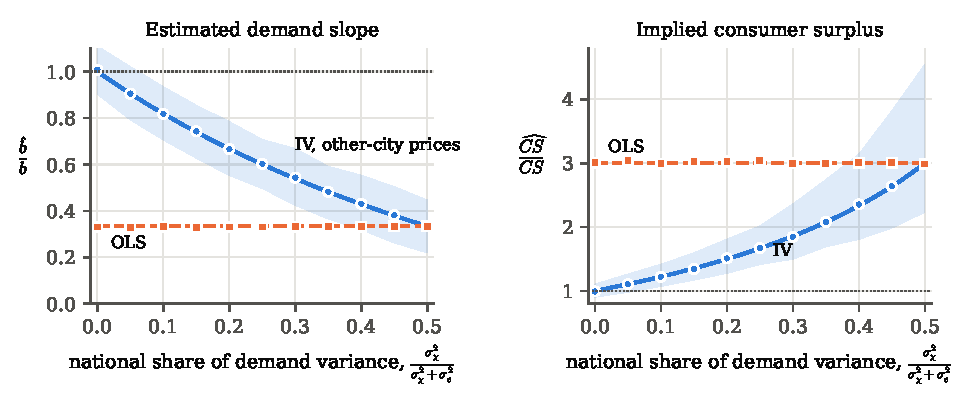
\includegraphics[width=\textwidth]{figures/ch10/hausman_iv_bias.pdf}
\caption{Hausman instruments with national demand shocks, a Monte Carlo experiment. The left panel shows the
estimated demand slope relative to the truth. The right panel shows the implied consumer surplus with linear
demand relative to the truth. Markers are Monte Carlo means (slope) or medians (surplus) over 500
replications. Lines are the probability limits of \cref{prop:10-hausman-iv-bias}, solid for IV and dashed for
OLS. The band shows the 10th to 90th percentiles of the IV estimates. The design has 7 cities, 137 weeks,
$b = 2$, $\sigma_\chi^2 + \sigma_e^2 = 1$ and $\sigma_k = \sigma_v = 0.5$. All shocks are anticipated, and city
fixed effects are removed. The script is \texttt{figures/ch10/src/hausman\_iv\_bias.py}.}
\label{fig:10-hausman-iv-mc}
\end{figure}

Two features of the experiment deserve comment. First, the instrument is strong throughout: the correlation
between a city's price and the other-city average is about 0.5 to 0.65. A strong first stage is no
protection against an invalid instrument. Second, week fixed effects cannot remove the problem for a single
product. They would absorb the national cost shocks as well, and with them all identifying variation. In a
system with many brands, week effects common to all brands absorb only aggregate shocks. Brand-specific
national shocks, the kind Bresnahan describes, remain.

\casehead{Evidence from later work}
\citet{Nevo2001} uses Hausman instruments for cereal in a random-coefficients model (\cref{ch:blp}). His
instruments are regional quarterly average prices of the same brand, excluding the city being instrumented
(p.~321). He discusses exactly Bresnahan's concern. A national demand shock, such as the discovery that fiber
reduces the risk of cancer, would raise the valuation of fiber-rich brands in all cities and violate the
assumption. He argues that the concern is weaker for well-established brands and that time dummies absorb
aggregate shocks. He then compares the price coefficient across instrument sets in his logit regressions
(Table V). With other-city prices it is $-17.57$ (0.50), and with proxies for local marginal cost it is
$-17.12$ (0.49), against $-7.26$ (0.16) by OLS with brand dummies. The two instrument sets agree. Nevo notes,
however, that regional demand shocks would invalidate both, and overidentification tests reject in all
columns except the one with city fixed effects. The comparison is informative, but it cannot rule out
brand-specific national shocks.

\subsection{Imperfect competition is ``off point''}\label{sec:10-bresnahan-competition}

Bresnahan's second criticism concerns economic interpretation (pp.~243--246). Imperfect competition links
new goods and market power in three ways. A new good can create market power for its inventor. It can
destroy market power of competing products. And the transitory market power that results is a reward that
motivates invention.

\casehead{Private returns}
The steep $dd$ that implies a large consumer surplus also implies a large monopoly rent if one firm owns the
product (p.~243). \Cref{rem:10-steep} makes this exact for linear demand, where consumer surplus at the
monopoly price is half the profit. Demand studies of new goods therefore speak to private returns to
innovation as well as social returns. With multiproduct firms and competitive responses, the calculation
needs the whole demand system and a supply model (p.~243).

\casehead{Rivals' prices}
Under imperfect competition among single-product firms, a new product lowers the market power of existing
products and so lowers prices (p.~243). This is one of the classical benefits of competition.
\Cref{sec:10-rival-prices} develops the argument. It proves the result for logit demand
(\cref{prop:10-logit-rivals}) and discusses Bresnahan's two qualifications, that unusual elasticities can
reverse it (fn.~12) and that Bertrand competition reinforces the direct effects (fn.~13).

Hausman holds the prices of Kellogg and Post fixed. Bresnahan calls this ``a common error among those who
are new to models of imperfect competition, but an important one'' (p.~244). The Bertrand solution concept
has firms maximize post-entry profits taking each other's post-entry prices as given. The analyst who
computes the effect of entry cannot take those prices as given, because entry changes the game. Typically
the rivals' prices fall. By holding them fixed, Hausman solves the price-discrimination problem of General
Mills as if it were a monopolist. His claim of a lower bound is therefore wrong, as Hausman's own fn.~32
partly concedes.

\casehead{The multiproduct firm's own prices}
Even for General Mills alone, the direction of the price change is ambiguous. Adding a brand changes the
first-order condition \eqref{eq:10-foc-elast} for an existing brand $j$ in the three ways of
\cref{sec:10-own-prices} (pp.~244--245). The new brand's term favors a higher $p_j$, which is the effect
Hausman stresses. Bresnahan counts the falls in the revenue shares of the existing brands, $w_j$ among them,
as the offsetting effects. At fixed margins and elasticities, only the cannibalization of the firm's other
brands pushes the other way, because it shrinks the positive cross terms. Bresnahan states that with linear demand and a two-product firm the effects exactly offset, and
\cref{prop:10-linear-offset} proves this for any number of products. Any dominance of one effect therefore
comes ``from higher-order derivatives'', and the paper offers no evidence on them (p.~245). The reproduction of Table 5.7 in
\cref{sec:10-hausman-imperfect} makes the point concrete. Hausman's ``without'' margins keep the post-launch
shares of Cheerios and Honey-Nut, so they include the first effect and omit the second and third.

\casehead{Where the action is}
Bresnahan summarizes the possibilities in the two-by-two classification of \cref{tab:10-bresnahan-2x2}.
Hausman's analysis sits in the price-discrimination cell. Bresnahan argues that if the social return is the object of interest, Hausman ``has
quantified the generally far less important effect'' (p.~246). The competition cell, the effect of a new
good on the pricing incentives of rival firms, must in general be much more important.

\casehead{Conclusion}
Bresnahan was left ``unconvinced by key econometric assumptions'' and found the imperfect-competition
analysis ``off point''. To doubt the large single-product surplus may simply be to believe in nationwide
brand-name demand shocks. ``The puzzle of the value of this incremental product introduction remains
unsolved'' (p.~246).

\subsection{Assessment}\label{sec:10-bresnahan-assessment}

Each side of the exchange got something right. Hausman showed that the exact value of a new brand can be
computed from estimated demand, and that a flexible system can deliver a finite virtual price. He also showed
that the answer depends on market structure. Bresnahan showed that the identifying assumption is strong
exactly where the conclusion is sensitive. Own-price slopes biased toward zero produce steep $dd$ curves and
large surplus. He also showed that holding rivals' prices fixed answers a monopoly question, and that the
multiproduct effect itself is ambiguous.

Several kinds of evidence could settle the dispute. Price and quantity data spanning the launch would allow
a direct before-and-after comparison, which Hausman lacked. \citet{HausmanLeonard2002} later made such a
comparison for Kleenex Bath Tissue (KBT), which Kimberly-Clark rolled out across U.S. cities in waves.\footnote{We
checked the numbers in this paragraph against the authors' revised manuscript dated September 1999 (pp.~10--15 and
33--36, and Tables~2, 6 and~7), which thanks the journal's referees and editor. We did not check the published article, whose
page and table numbers may differ.}
They use weekly Nielsen scanner data on the seven largest brands in 30 cities from January 1992 to September 1995.
KBT was already sold in 17 cities when the data begin. It entered three more in July 1993 and the last ten in May
1994. For each incumbent brand they estimate by ordinary least squares
\begin{equation}\label{eq:10-hl-direct}
  \ln p_{ct} = \lambda_c + \omega_t + \beta_1 I_{ct} + \beta_2 M_{ct} + e_{ct},
\end{equation}
where $c$ indexes cities and $t$ weeks, and $\lambda_c$ and $\omega_t$ are city and week fixed effects. The
indicator $I_{ct}$ equals one once KBT is sold in city $c$, and $M_{ct}$ marks the third-wave cities in the weeks
between the second and third waves. The staggered entry separates $\beta_1$ from the common shocks absorbed by
$\omega_t$. All six estimated price effects are negative (Table~2). Cottonelle fell 8.2 percent (standard error
1.3), Charmin and Angel Soft 3.5 percent, private label 3.8 percent and Northern 2.3 percent. The economy brand
ScotTissue fell only 0.6 percent (0.5). Kimberly-Clark had almost no prior share, so this is the competition cell
of Bresnahan's classification, and the prices of rivals fell as he predicts. The authors also predict these
changes from the post-entry demand system under Nash-Bertrand pricing. The predictions are close for four brands
but well short for Cottonelle ($-3.6$ percent) and private label ($-0.7$ percent), where $t$-tests reject equality
(Table~6). Because the comparison gives mixed support, they describe their evidence for Nash-Bertrand pricing as
cautious. The authors put the total consumer
gain at \$69.2 million a year, 7.3 percent of bath tissue spending in the 30 cities (Table~7). About half of it
comes from the lower prices of existing brands (p.~36).
Residuals of the same brand in different cities and the same week can be tested for correlation, the most
direct symptom of national shocks. Overidentification tests across cities, which fn.~20 of Hausman's paper
proposes, could be reported. Instruments from observed local costs offer a comparison, as in
\citet{Nevo2001}. Each check addresses a specific threat. None is a general proof of validity.

The broader literature moved in two directions. One kept product-space demand and looked for better
instruments and data. The other moved to characteristics space \citep{Berry1994,BerryLevinsohnPakes1995}.
There the value of a new product depends on its location relative to existing products, and instruments come
from the characteristics of rivals. That approach has its own extrapolation problem, the idiosyncratic
taste shock that gives every product a positive value, which \cref{sec:10-charspace} analyzes. It also has its
own instrument problem, the assumption that characteristics are exogenous (\cref{ch:discrete}).
\citet{Petrin2002}, studied in \cref{sec:10-petrin}, combines characteristics-space demand with micro data and
recomputes the full Bertrand equilibrium without the new product. His results quantify the competition cell of
Bresnahan's classification, together with the price-discrimination cell.
